% Preambel mit Einstellungen importieren
% Document type and used packages
\documentclass[open=right, % Kapitel darf nur auf rechten Seite beginnen
    paper=A4,               % DIN-A4-Papier
    a4paper,                % DIN-A4-Papier
    12pt,                   % Schriftgöße
    headings=small,         % Kleine Überschriften
    headsepline=true,       % Trennlinie am Kopf der Seite
    footsepline=false,      % Keine Trennlinie am Fuß der Seite
    bibliography=totoc,     % Literaturverzeichnis in das Inhaltsverzeichnis aufnehmen
    twoside=on,             % Doppelseitiger Druck - auf off stellen für einseitig
    DIV=7,                  % Verhältnis der Ränder zum bedruckten Bereich
    chapterprefix=true,     % Kapitel x vor dem Kapitelnamen
    cleardoublepage=plain]{scrbook}

% Pakete einbinden, die benötigt werden
\usepackage{scrpage2}
\usepackage[utf8]{inputenc}       % Dateien in UTF-8 benutzen
\usepackage[T1]{fontenc}          % Zeichenkodierung
\usepackage{graphicx}             % Bilder einbinden
\usepackage[main=ngerman, english]{babel}       % Deutsch und Englisch unterstützen
\usepackage{xcolor}               % Color support
\usepackage{amsmath}              % Matheamtische Formeln
\usepackage{amsfonts}             % Mathematische Zeichensätze
\usepackage{amssymb}              % Mathematische Symbole
\usepackage{float}                % Fließende Objekte (Tabellen, Grafiken etc.)
\usepackage{booktabs}             % Korrekter Tabellensatz
\usepackage[printonlyused]{acronym}  % Abkürzungsverzeichnis [nur verwendete Abkürzugen]
\usepackage{makeidx}              % Sachregister
\usepackage{listings}             % Source Code listings
\usepackage{listingsutf8}         % Listings in UTF8
\usepackage[hang,font={sf,footnotesize},labelfont={footnotesize,bf}]{caption} % Beschriftungen
\usepackage[scaled]{helvet}       % Schrift Helvetia laden
\usepackage[absolute]{textpos}	  % Absolute Textpositionen (für Deckblatt)
\usepackage{calc}                 % Berechnung von Positionen
\usepackage{blindtext}            % Blindtexte
\usepackage[bottom=40mm,left=35mm,right=35mm,top=30mm]{geometry} % Ränder ändern
\usepackage{setspace}             % Abstände korrigieren
\usepackage{ifthen}               % Logische Bedingungen mit ifthenelse
\usepackage{scrhack}              % Get rid of tocbasic warnings
\usepackage[pagebackref=false,german]{hyperref}  % Hyperlinks
\usepackage[all]{hypcap}          % Korrekte Verlinkung von Floats
\usepackage[autostyle=true,german=quotes]{csquotes}   % Zitate
\usepackage[backend=biber,
  isbn=false,                     % ISBN nicht anzeigen, gleiches geht mit nahezu allen anderen Feldern
  sortlocale=en_EN,               % Sortierung der Einträge für Deutsch
                                  %      de_DE: für Deutsch
                                  %      en_US: für Englisch
  autocite=inline,                % regelt Aussehen für \autocite
                                  %      inline: Zitat in Klammern (\parancite)
                                  %      footnote: Zitat in Fußnoten (\footcite)
                                  %      plain: Zitat direkt ohne Klammern (\cite)
  style=numeric,               % Legt den Stil für die Zitate fest
                                  %      ieee: Zitate als Zahlen [1]
                                  %      alphabetic: Zitate als Kürzel und Jahr [Ein05]
                                  %      authoryear: Zitate Author und Jahr [Einstein (1905)]
  hyperref=true,                  % Hyperlinks für Ziate
  citestyle=numeric,
]{biblatex}                       % Literaturverwaltung mit BibLaTeX
\usepackage{rotating}             % Seiten drehen
\usepackage{harveyballs}          % Harveyballs

\setlength{\bibitemsep}{1em}     % Abstand zwischen den Literaturangaben
\setlength{\bibhang}{2em}        % Einzug nach jeweils erster Zeile

% Trennung von URLs im Literaturverzeichnis (große Werte [> 10000] verhindern die Trennung)
\defcounter{biburlnumpenalty}{10} % Strafe für Trennung in URL nach Zahl
\defcounter{biburlucpenalty}{500}  % Strafe für Trennung in URL nach Großbuchstaben
\defcounter{biburllcpenalty}{500}  % Strafe für Trennung in URL nach Kleinbuchstaben

% Farben definieren
\definecolor{linkblue}{RGB}{0, 0, 100}
\definecolor{linkblack}{RGB}{0, 0, 0}
\definecolor{comment}{RGB}{63, 127, 95}
\definecolor{darkgreen}{RGB}{14, 144, 102}
\definecolor{darkblue}{RGB}{0,0,168}
\definecolor{darkred}{RGB}{128,0,0}
\definecolor{javadoccomment}{RGB}{0,0,240}

% Einstellungen für das Hyperlink-Paket
\hypersetup{
    colorlinks=true,      % Farbige links verwenden
%    allcolors=linkblue,
    linktoc=all,          % Links im Inhaltsverzeichnis
    linkcolor=linkblack,  % Querverweise
    citecolor=linkblack,  % Literaturangaben
	filecolor=linkblack,  % Dateilinks
	urlcolor=linkblack    % URLs
}

% Einstellungen für Quelltexte
\lstset{
      xleftmargin=0.2cm,
      basicstyle=\footnotesize\ttfamily,
      keywordstyle=\color{darkgreen},
      identifierstyle=\color{darkblue},
      commentstyle=\color{comment},
      stringstyle=\color{darkred},
      tabsize=2,
      lineskip={2pt},
      columns=flexible,
      inputencoding=utf8,
      captionpos=b,
      breakautoindent=true,
	  breakindent=2em,
	  breaklines=true,
	  prebreak=,
	  postbreak=,
      numbers=none,
      numberstyle=\tiny,
      showspaces=false,      % Keine Leerzeichensymbole
      showtabs=false,        % Keine Tabsymbole
      showstringspaces=false,% Leerzeichen in Strings
      morecomment=[s][\color{javadoccomment}]{/**}{*/},
      literate={Ö}{{\"O}}1 {Ä}{{\"A}}1 {Ü}{{\"U}}1 {ß}{{\ss}}2 {ü}{{\"u}}1 {ä}{{\"a}}1 {ö}{{\"o}}1
}

\urlstyle{same}

% Einstellungen für Überschriften
\renewcommand*{\chapterformat}{%
  \Large\chapapp~\thechapter   % Große Schrift
  \vspace{0.3cm}               % Abstand zum Titel des Kapitels
}

% Abstände für die Überschriften setzen
\renewcommand{\chapterheadstartvskip}{\vspace*{2.6cm}}
\renewcommand{\chapterheadendvskip}{\vspace*{1.5cm}}

\RedeclareSectionCommand[
  beforeskip=-1.8\baselineskip,
  afterskip=0.25\baselineskip]{section}

\RedeclareSectionCommand[
  beforeskip=-1.8\baselineskip,
  afterskip=0.15\baselineskip]{subsection}

\RedeclareSectionCommand[
  beforeskip=-1.8\baselineskip,
  afterskip=0.15\baselineskip]{subsubsection}


% In der Kopfzeile nur die kurze Kapitelbezeichnung (ohne Kapitel davor)
\renewcommand*\chaptermarkformat{\thechapter\autodot\enskip}
\automark[chapter]{chapter}

% Einstellungen für Schriftarten
\setkomafont{pagehead}{\normalfont\sffamily}
\setkomafont{pagenumber}{\normalfont\sffamily}
\setkomafont{paragraph}{\sffamily\bfseries\small}
\setkomafont{subsubsection}{\sffamily\itshape\bfseries\small}
\addtokomafont{footnote}{\footnotesize}
\setkomafont{chapter}{\LARGE\selectfont\bfseries}

% Wichtige Abstände
\setlength{\parskip}{0.2cm}  % 2mm Abstand zwischen zwei Absätzen
\setlength{\parindent}{0mm}  % Absätze nicht einziehen
\clubpenalty = 10000         % Keine "Schusterjungen"
\widowpenalty = 10000        % Keine "Hurenkinder"
\displaywidowpenalty = 10000 % Keine "Hurenkinder"
\renewcommand{\footnotesize}{\fontsize{9}{10}\selectfont} % Größe der Fußnoten
\setlength{\footnotesep}{8pt} % Abstand zwischen den Fußnoten

% Index erzeugen
\makeindex

% Einfacher Font-Wechsel über dieses Makro
\newcommand{\changefont}[3]{
\fontfamily{#1} \fontseries{#2} \fontshape{#3} \selectfont}

% Eigenes Makro für Bilder
\newcommand{\bild}[3]{
\begin{figure}[h]
  \centering
  \includegraphics[width=#2]{#1}
  \caption{#3}
  \label{#1}
\end{figure}}

% Wo liegt Sourcecode?
\newcommand{\srcloc}{src/}

% Wo sind die Bilder?
\graphicspath{{bilder/}}

% Makros für typographisch korrekte Abkürzungen
\newcommand{\zb}[0]{z.\,B.\ }
\newcommand{\dahe}[0]{d.\,h.\ }
\newcommand{\ua}[0]{u.\,a.\ }

% Flags für Veröffentlichung und Sperrvermerk
\newboolean{hsmapublizieren}
\newboolean{hsmasperrvermerk}

% Dokumenteninfos importieren
\newcommand{\hsmasprache}{en} 
\newcommand{\hsmatitelde}{Modellierung virtueller Umgebungen für Roboterexperimente}

\newcommand{\hsmatitelen}{Modeling virtual environments for robot experiments}
\newcommand{\hsmaort}{Mannheim}
\newcommand{\hsmaautorvname}{Moritz Laurin}
\newcommand{\hsmaautornname}{Thomas}
\newcommand{\hsmadatum}{27.11.2018}
\newcommand{\hsmajahr}{2018}
\newcommand{\hsmabetreuer}{Prof. Thomas Ihme, Hochschule Mannheim}
\newcommand{\hsmazweitkorrektor}{N/A, N/A}
\newcommand{\hsmafakultaet}{I}
\newcommand{\hsmastudiengang}{IB}

\setboolean{hsmapublizieren}{true}
\setboolean{hsmasperrvermerk}{false}

% Literatur-Datenbank
\addbibresource{literatur.bib} %Imports bibliography file

\begin{document}
\frontmatter

% Römische Ziffern für die "Front-Matter"
\setcounter{page}{0}
\changefont{ptm}{m}{n}  % Times New Roman für den Fließtext
\renewcommand{\rmdefault}{ptm}

% Titelblatt
% -------------------------------------------------------
% In dieser Datei sollten eigentlich keine Veränderungen mehr
% notwendig sein.
% -------------------------------------------------------

\thispagestyle{empty}

% Fakultäten der HS-Mannheim
% -------------------------------------------------------
\ifthenelse{\equal{\hsmafakultaet}{I}}%
  {\newcommand{\hsmafakultaetlangde}{Fakultät für Informatik}%
   \newcommand{\hsmafakultaetlangen}{Department of Computer Science}}{}

\ifthenelse{\equal{\hsmafakultaet}{E}}%
  {\newcommand{\hsmafakultaetlangde}{Fakultät für Elektrotechnik}%
   \newcommand{\hsmafakultaetlangen}{Department of Electrical Engineering}}{}

\ifthenelse{\equal{\hsmafakultaet}{S}}%
  {\newcommand{\hsmafakultaetlangde}{Fakultät für Sozialwesen}%
   \newcommand{\hsmafakultaetlangen}{Department of Social Work}}{}
   
\ifthenelse{\equal{\hsmafakultaet}{B}}%
  {\newcommand{\hsmafakultaetlangde}{Fakultät für Biotechnologie}%
   \newcommand{\hsmafakultaetlangen}{Department of Biotechnology}}{}

\ifthenelse{\equal{\hsmafakultaet}{D}}%
  {\newcommand{\hsmafakultaetlangde}{Fakultät für Gestaltung}%
   \newcommand{\hsmafakultaetlangen}{Department of Design}}{}

\ifthenelse{\equal{\hsmafakultaet}{M}}%
  {\newcommand{\hsmafakultaetlangde}{Fakultät für Maschinenbau}%
   \newcommand{\hsmafakultaetlangen}{Department of Mechanical Engineering}}{}

\ifthenelse{\equal{\hsmafakultaet}{N}}%
  {\newcommand{\hsmafakultaetlangde}{Fakultät für Informationstechnik}%
   \newcommand{\hsmafakultaetlangen}{Department of Information Technology}}{}
   
\ifthenelse{\equal{\hsmafakultaet}{W}}%
  {\newcommand{\hsmafakultaetlangde}{Fakultät für Wirtschaftsingenieurwesen}%
   \newcommand{\hsmafakultaetlangen}{Department of Engineering and Management}}{}
   
\ifthenelse{\equal{\hsmafakultaet}{C}}%
  {\newcommand{\hsmafakultaetlangde}{Fakultät für Verfahrens- und Chemietechnik}%
   \newcommand{\hsmafakultaetlangen}{Department of Chemical Process Engineering}}{}
   

\ifthenelse{\equal{\hsmastudiengang}{IB}}%
  {\newcommand{\hsmastudienganglangde}{Informatik}%
  \newcommand{\hsmastudienganglangen}{Computer Science}%
  \newcommand{\hsmatypde}{Bachelor-Thesis}%
  \newcommand{\hsmatypen}{Bachelor Thesis}%
  \newcommand{\hsmagrad}{\hsmabsc}}{}

\ifthenelse{\equal{\hsmastudiengang}{IMB}}%
  {\newcommand{\hsmastudienganglangde}{Medizinische Informatik}%
  \newcommand{\hsmastudienganglangen}{Medical Informatics}%
  \newcommand{\hsmatypde}{Bachelor-Thesis}%
  \newcommand{\hsmatypen}{Bachelor Thesis}%
  \newcommand{\hsmagrad}{\hsmabsc}}{}
  
\ifthenelse{\equal{\hsmastudiengang}{UIB}}%
  {\newcommand{\hsmastudienganglangde}{Unternehmens- und Wirtschaftsinformatik}%
  \newcommand{\hsmastudienganglangen}{Enterprise Computing}%  
  \newcommand{\hsmatypde}{Bachelor-Thesis}%
  \newcommand{\hsmatypen}{Bachelor Thesis}%
  \newcommand{\hsmagrad}{\hsmabsc}}{}

\ifthenelse{\equal{\hsmastudiengang}{IM}}%
  {\newcommand{\hsmastudienganglangde}{Informatik}%
   \newcommand{\hsmastudienganglangen}{Computer Science}%
   \newcommand{\hsmatypde}{Master-Thesis}%
   \newcommand{\hsmatypen}{Master Thesis}%
   \newcommand{\hsmagrad}{\hsmamaster}}{}

\ifthenelse{\equal{\hsmastudiengang}{MEB}}%
  {\newcommand{\hsmastudienganglangde}{Mechatronik}%
   \newcommand{\hsmastudienganglangen}{Mechatronic}%
   \newcommand{\hsmatypde}{Bachelor-Thesis}%
   \newcommand{\hsmatypen}{Bachelor Thesis}%
   \newcommand{\hsmagrad}{\hsmabsc}}{}
   
\ifthenelse{\equal{\hsmastudiengang}{UB}}%
  {\newcommand{\hsmastudienganglangde}{Automatisierungstechnik}%
   \newcommand{\hsmastudienganglangen}{Automation Technology}%
   \newcommand{\hsmatypde}{Bachelor-Thesis}%
   \newcommand{\hsmatypen}{Bachelor Thesis}%
   \newcommand{\hsmagrad}{\hsmabsc}}{}
   
\ifthenelse{\equal{\hsmastudiengang}{ELB}}%
  {\newcommand{\hsmastudienganglangde}{Elektro- und Informationstechnik/Ingenieurpädagogik}%
   \newcommand{\hsmastudienganglangen}{Elektro- und Informationstechnik/Ingenieurpädagogik}%
   \newcommand{\hsmatypde}{Bachelor-Thesis}%
   \newcommand{\hsmatypen}{Bachelor Thesis}%
   \newcommand{\hsmagrad}{\hsmabsc}}{} 
   
\ifthenelse{\equal{\hsmastudiengang}{EBE}}%
  {\newcommand{\hsmastudienganglangde}{Energietechnik und erneuerbare Energien}%
   \newcommand{\hsmastudienganglangen}{Power Engineering ans Renewable Energies}%
   \newcommand{\hsmatypde}{Bachelor-Thesis}%
   \newcommand{\hsmatypen}{Bachelor Thesis}%
   \newcommand{\hsmagrad}{\hsmabsc}}{}

\ifthenelse{\equal{\hsmastudiengang}{TS}}%
  {\newcommand{\hsmastudienganglangde}{Translation Studies}%
   \newcommand{\hsmastudienganglangen}{Translation Studies}%
   \newcommand{\hsmatypde}{Bachelor-Thesis}%
   \newcommand{\hsmatypen}{Bachelor Thesis}%
   \newcommand{\hsmagrad}{\hsmabsc}}{}
  
\ifthenelse{\equal{\hsmastudiengang}{EM}}%
  {\newcommand{\hsmastudienganglangde}{Automatisierungs- und Energiesysteme}%
   \newcommand{\hsmastudienganglangen}{Automation and Energy Systems}%
   \newcommand{\hsmatypde}{Master-Thesis}%
   \newcommand{\hsmatypen}{Master Thesis}%
   \newcommand{\hsmagrad}{\hsmamaster}}{}
   
\ifthenelse{\equal{\hsmastudiengang}{ELM}}%
  {\newcommand{\hsmastudienganglangde}{Lehramt Ingenieurpädagogik}%
   \newcommand{\hsmastudienganglangen}{Lectureship Educational Engineering}%
   \newcommand{\hsmatypde}{Master-Thesis}%
   \newcommand{\hsmatypen}{Master Thesis}%
   \newcommand{\hsmagrad}{\hsmamaster}}{}
   
\ifthenelse{\equal{\hsmastudiengang}{SAB}}%
  {\newcommand{\hsmastudienganglangde}{Soziale Arbeit}%
   \newcommand{\hsmastudienganglangen}{Social Labour}%
   \newcommand{\hsmatypde}{Bachelor-Thesis}%
   \newcommand{\hsmatypen}{Bachelor Thesis}%
   \newcommand{\hsmagrad}{\hsmaba}}{}
   
\ifthenelse{\equal{\hsmastudiengang}{SAM}}%
  {\newcommand{\hsmastudienganglangde}{Soziale Arbeit}%
   \newcommand{\hsmastudienganglangen}{Social Labour}%
   \newcommand{\hsmatypde}{Master-Thesis}%
   \newcommand{\hsmatypen}{Master Thesis}%
   \newcommand{\hsmagrad}{\hsmamastera}}{}
   
\ifthenelse{\equal{\hsmastudiengang}{BB}}%
  {\newcommand{\hsmastudienganglangde}{Biotechnology}%
   \newcommand{\hsmastudienganglangen}{Biotechnology}%
   \newcommand{\hsmatypde}{Bachelor-Thesis}%
   \newcommand{\hsmatypen}{Bachelor Thesis}%
   \newcommand{\hsmagrad}{\hsmabsc}}{}
   
\ifthenelse{\equal{\hsmastudiengang}{BCB}}%
  {\newcommand{\hsmastudienganglangde}{Biologische Chemie}%
   \newcommand{\hsmastudienganglangen}{Biological Chemics}%
   \newcommand{\hsmatypde}{Bachelor-Thesis}%
   \newcommand{\hsmatypen}{Bachelor Thesis}%
   \newcommand{\hsmagrad}{\hsmabsc}}{}
   
\ifthenelse{\equal{\hsmastudiengang}{BMEBST}}%
  {\newcommand{\hsmastudienganglangde}{Biotechnology - Biomedical Science and Technology}%
   \newcommand{\hsmastudienganglangen}{Biotechnology - Biomedical Science and Technology}%
   \newcommand{\hsmatypde}{Master-Thesis}%
   \newcommand{\hsmatypen}{Master Thesis}%
   \newcommand{\hsmagrad}{\hsmamaster}}{}
   
\ifthenelse{\equal{\hsmastudiengang}{BMEBPD}}%
  {\newcommand{\hsmastudienganglangde}{Biotechnology - Bioprocess Development}%
   \newcommand{\hsmastudienganglangen}{Biotechnology - Bioprocess Development}%
   \newcommand{\hsmatypde}{Master-Thesis}%
   \newcommand{\hsmatypen}{Master Thesis}%
   \newcommand{\hsmagrad}{\hsmamaster}}{}
   
\ifthenelse{\equal{\hsmastudiengang}{BLSM}}%
  {\newcommand{\hsmastudienganglangde}{Life Science Management}%
   \newcommand{\hsmastudienganglangen}{Life Science Management}%
   \newcommand{\hsmatypde}{Master-Thesis}%
   \newcommand{\hsmatypen}{Master Thesis}%
   \newcommand{\hsmagrad}{\hsmamaster}}{}
   
\ifthenelse{\equal{\hsmastudiengang}{KDB}}%
  {\newcommand{\hsmastudienganglangde}{Kommunikationsdesign}%
   \newcommand{\hsmastudienganglangen}{Communication Design}%
   \newcommand{\hsmatypde}{Bachelor-Thesis}%
   \newcommand{\hsmatypen}{Bachelor Thesis}%
   \newcommand{\hsmagrad}{\hsmaba}}{}
   
\ifthenelse{\equal{\hsmastudiengang}{KDM}}%
  {\newcommand{\hsmastudienganglangde}{Kommunikationsdesign}%
   \newcommand{\hsmastudienganglangen}{Communication Design}%
   \newcommand{\hsmatypde}{Master-Thesis}%
   \newcommand{\hsmatypen}{Master Thesis}%
   \newcommand{\hsmagrad}{\hsmamastera}}{}
   
\ifthenelse{\equal{\hsmastudiengang}{MB}}%
  {\newcommand{\hsmastudienganglangde}{Maschinenbau}%
   \newcommand{\hsmastudienganglangen}{Mechanical Engineering}%
   \newcommand{\hsmatypde}{Bachelor-Thesis}%
   \newcommand{\hsmatypen}{Bachelor Thesis}%
   \newcommand{\hsmagrad}{\hsmabsc}}{}
   
\ifthenelse{\equal{\hsmastudiengang}{MM}}%
  {\newcommand{\hsmastudienganglangde}{Maschinenbau}%
   \newcommand{\hsmastudienganglangen}{Mechanical Engineering}%
   \newcommand{\hsmatypde}{Master-Thesis}%
   \newcommand{\hsmatypen}{Master Thesis}%
   \newcommand{\hsmagrad}{\hsmamaster}}{}
   
\ifthenelse{\equal{\hsmastudiengang}{NEB}}%
  {\newcommand{\hsmastudienganglangde}{Elektronik}%
   \newcommand{\hsmastudienganglangen}{Electronics}%
   \newcommand{\hsmatypde}{Bachelor-Thesis}%
   \newcommand{\hsmatypen}{Bachelor Thesis}%
   \newcommand{\hsmagrad}{\hsmabsc}}{}
   
\ifthenelse{\equal{\hsmastudiengang}{TIB}}%
  {\newcommand{\hsmastudienganglangde}{Technische Informatik}%
   \newcommand{\hsmastudienganglangen}{Technical Information Technology}%
   \newcommand{\hsmatypde}{Bachelor-Thesis}%
   \newcommand{\hsmatypen}{Bachelor Thesis}%
   \newcommand{\hsmagrad}{\hsmabsc}}{}
   
\ifthenelse{\equal{\hsmastudiengang}{MTB}}%
  {\newcommand{\hsmastudienganglangde}{Medizintechnik}%
   \newcommand{\hsmastudienganglangen}{Medical Technology}%
   \newcommand{\hsmatypde}{Bachelor-Thesis}%
   \newcommand{\hsmatypen}{Bachelor Thesis}%
   \newcommand{\hsmagrad}{\hsmabsc}}{}
   
\ifthenelse{\equal{\hsmastudiengang}{MTM}}%
  {\newcommand{\hsmastudienganglangde}{Medizintechnik}%
   \newcommand{\hsmastudienganglangen}{Medical Technology}%
   \newcommand{\hsmatypde}{Master-Thesis}%
   \newcommand{\hsmatypen}{Master Thesis}%
   \newcommand{\hsmagrad}{\hsmamaster}}{}
   
\ifthenelse{\equal{\hsmastudiengang}{NM}}%
  {\newcommand{\hsmastudienganglangde}{Informationstechnik}%
   \newcommand{\hsmastudienganglangen}{Informationstechnik}%
   \newcommand{\hsmatypde}{Master-Thesis}%
   \newcommand{\hsmatypen}{Master Thesis}%
   \newcommand{\hsmagrad}{\hsmamaster}}{}
   
\ifthenelse{\equal{\hsmastudiengang}{WB}}%
  {\newcommand{\hsmastudienganglangde}{Wirtschaftsingenieurwesen}%
   \newcommand{\hsmastudienganglangen}{Business Administration and Engineering}%
   \newcommand{\hsmatypde}{Bachelor-Thesis}%
   \newcommand{\hsmatypen}{Bachelor Thesis}%
   \newcommand{\hsmagrad}{\hsmabsc}}{}
   
\ifthenelse{\equal{\hsmastudiengang}{WM}}%
  {\newcommand{\hsmastudienganglangde}{Wirtschaftsingenieurwesen}%
   \newcommand{\hsmastudienganglangen}{Business Administration and Engineering}%
   \newcommand{\hsmatypde}{Master-Thesis}%
   \newcommand{\hsmatypen}{Master Thesis}%
   \newcommand{\hsmagrad}{\hsmamaster}}{}
   
\ifthenelse{\equal{\hsmastudiengang}{VB}}%
  {\newcommand{\hsmastudienganglangde}{Verfahrenstechnik}%
   \newcommand{\hsmastudienganglangen}{Process Engineering}%
   \newcommand{\hsmatypde}{Bachelor-Thesis}%
   \newcommand{\hsmatypen}{Bachelor Thesis}%
   \newcommand{\hsmagrad}{\hsmabsc}}{}
   
\ifthenelse{\equal{\hsmastudiengang}{CB}}%
  {\newcommand{\hsmastudienganglangde}{Chemische Technik}%
   \newcommand{\hsmastudienganglangen}{Chemical Engineering}%
   \newcommand{\hsmatypde}{Bachelor-Thesis}%
   \newcommand{\hsmatypen}{Bachelor Thesis}%
   \newcommand{\hsmagrad}{\hsmabsc}}{}
   
\ifthenelse{\equal{\hsmastudiengang}{CM}}%
  {\newcommand{\hsmastudienganglangde}{Chemieingenieurwesen}%
   \newcommand{\hsmastudienganglangen}{Chemical Engineering}%
   \newcommand{\hsmatypde}{Master-Thesis}%
   \newcommand{\hsmatypen}{Master Thesis}%
   \newcommand{\hsmagrad}{\hsmamaster}}{}

\newcommand{\hsmabsc}{Bachelor of Science (B.Sc.)}
\newcommand{\hsmaba}{Bachelor of Arts (B.A.)}
\newcommand{\hsmamaster}{Master of Science (M.Sc.)}
\newcommand{\hsmamastera}{Master of Arts (M.A.)}
\newcommand{\hsmamasterba}{Master of Business Administration (MBA)}

\newcommand{\hsmakoerperschaftde}{Hochschule Mannheim}
\newcommand{\hsmakoerperschaften}{University of Applied Sciences Mannheim}

\newcommand{\hsmaautorbib}{\hsmaautornname, \hsmaautorvname} % Autor Nachname, Vorname
\newcommand{\hsmaautor}{\hsmaautorvname \ \hsmaautornname} % Autor Vorname Nachname

\ifthenelse{\equal{\hsmasprache}{de}}%
  {\newcommand{\hsmatyp}{\hsmatypde}%
   \newcommand{\hsmathesistype}{zur Erlangung des akademischen Grades \hsmagrad}%
   \newcommand{\hsmakoerperschaft}{\hsmakoerperschaftde}%
   \newcommand{\hsmastudiengangname}{Studiengang \hsmastudienganglangde}%
   \newcommand{\hsmastudienganglang}{\hsmastudienganglangde}%
   \newcommand{\hsmatitel}{\hsmatitelde}%
   \newcommand{\hsmatutor}{Betreuer}%
   \newcommand{\hsmafakultaetlang}{\hsmafakultaetlangde}%
   \newcommand{\hsmalistoftables}{Tabellenverzeichnis}%
   \newcommand{\hsmalistoffigures}{Abbildungsverzeichnis}%
   \newcommand{\hsmalistings}{Quellcodeverzeichnis}%
   \newcommand{\hsmaindex}{Index}%
   \newcommand{\hsmaabbreviations}{Abkürzungsverzeichnis}%   
   \selectlanguage{ngerman}}%
  {\newcommand{\hsmatyp}{\hsmatypen}%
   \newcommand{\hsmathesistype}{for the acquisition of the academic degree \hsmagrad}%
   \newcommand{\hsmakoerperschaft}{\hsmakoerperschaften}%
   \newcommand{\hsmastudiengangname}{Course of Studies: \hsmastudienganglang}%
   \newcommand{\hsmastudienganglang}{\hsmastudienganglangen}%
   \newcommand{\hsmatitel}{\hsmatitelen}%
   \newcommand{\hsmatutor}{Tutors}
   \newcommand{\hsmafakultaetlang}{\hsmafakultaetlangen}%
   \newcommand{\hsmalistoftables}{List of Tables}%
   \newcommand{\hsmalistoffigures}{List of Figures}%
   \newcommand{\hsmalistings}{Listings}%
   \newcommand{\hsmaindex}{Index}%
   \newcommand{\hsmaabbreviations}{List of Abbreviations}%
   \selectlanguage{english}}%


% Daten in die Standard-Felder von KOMA-Script eintragen
\titlehead{\hsmatyp\ in\  \hsmastudienganglang}
\subject{}
\title{\hsmatitel}
\author{\hsmaauthor}
\date{\small{\hsmadatum}}

% Daten für das fertige PDF-Dokument
\hypersetup{
  pdftitle={\hsmatitel},  % Titel des Dokuments
  pdfauthor={\hsmaautor},              % Autor
  pdfsubject={\hsmatyp\ in\ \hsmastudienganglang},                % Thema
  pdfkeywords={\hsmatitel}         % Schlüsselworte
}

\newlength{\bindekorrektur}
\newlength{\seitenanfang}
\newlength{\seitenbreite}
  
\setlength{\bindekorrektur}{-46mm}   % Korrektur der horizontalen Position
\setlength{\seitenanfang}{0mm}       % Korrektur der vertikalen Position
\setlength{\seitenbreite}{297mm}

\noindent
\includegraphics[width=7cm]{tex/img/hsma-logo.pdf}\\

% Titel der Arbeit
\begin{textblock*}{128mm}(45mm,\seitenanfang + 62mm) % 4,5cm vom linken Rand und 6,0cm vom oberen Rand
  \centering\Large\sffamily
  \vspace{4mm} % Kleiner zusätzlicher Abstand oben für bessere Optik
  \textbf{\hsmatitel}
\end{textblock*}%

% Name
\begin{textblock*}{128mm}(45mm,\seitenanfang + 103mm)
  \centering\large\sffamily
  \hsmaautor
\end{textblock*}

% Thesis
\begin{textblock*}{\seitenbreite}(\bindekorrektur,\seitenanfang + 130mm)
  \centering\large\sffamily
  \hsmatyp\\
  \begin{small}\hsmathesistype \end{small}\\
  \vspace{2mm}
  \hsmastudiengangname
\end{textblock*}

% Fakultät
\begin{textblock*}{\seitenbreite}(\bindekorrektur,\seitenanfang + 165mm)
  \centering\large\sffamily
  \hsmafakultaetlang\\
  \vspace{2mm}
  \hsmakoerperschaft
\end{textblock*}

% Datum
\begin{textblock*}{\seitenbreite}(\bindekorrektur,\seitenanfang + 190mm)
  \centering\large 
  \textsf{\hsmadatum}
\end{textblock*}

% Firma
\begin{textblock*}{\seitenbreite}(\bindekorrektur,\seitenanfang + 215mm)
  \centering\large 
  %\textsf{Durchgeführt bei der Firma \hsmafirma}
\end{textblock*}

% Betreuer
\begin{textblock*}{\seitenbreite}(\bindekorrektur,\seitenanfang + 240mm)
  \centering\large\sffamily
  \hsmatutor \\
  \vspace{2mm}
  \hsmabetreuer\\
  \vspace{2mm}
  \hsmazweitkorrektor
\end{textblock*}

% Bibliographische Informationen
\null\newpage
\thispagestyle{empty}
  
\newcommand{\hsmabibde}{\begin{small}\textbf{\hsmaautorbib}: \\ \hsmatitelde \ / \hsmaautor. \ -- \\ \hsmatypde, \hsmaort : \hsmakoerperschaftde, \hsmajahr. \pageref{lastpage} Seiten.\end{small}}

\newcommand{\hsmabiben}{\begin{small}\textbf{\hsmaautorbib}: \\ \hsmatitelen \ / \hsmaautor. \ -- \\ \hsmatypen, \hsmaort : \hsmakoerperschaften, \hsmajahr. \pageref{lastpage} pages. \end{small}}

\ifthenelse{\equal{\hsmasprache}{de}}%
  {\hsmabibde \\ \vspace{0.5cm} \\ \hsmabiben}
  {\hsmabiben \\ \vspace{0.5cm} \\ \hsmabibde}


% Erklärung
\clearpage\setcounter{page}{1}
\thispagestyle{empty}
\textsf{\large\textbf{Erklärung}}

Hiermit erkläre ich, dass ich die vorliegende Arbeit selbstständig verfasst und keine anderen als die angegebenen Quellen und Hilfsmittel benutzt habe.

\ifthenelse{\boolean{hsmapublizieren} \and \not\boolean{hsmasperrvermerk}}%
{
\vspace{0.5cm}
Ich bin damit einverstanden, dass meine Arbeit veröffentlicht wird, d.\,h. dass die Arbeit elektronisch gespeichert, in andere Formate konvertiert, auf den Servern der Hochschule Mannheim öffentlich zugänglich gemacht und über das Internet verbreitet werden darf. 
}{}%


\vspace{1cm}
\hsmaort, \hsmadatum \\

\vspace{1.2cm}						                                      
\hsmaautor

\ifthenelse{\boolean{hsmasperrvermerk}}%
{%
\vspace{11cm}
\color{red}\textsf{\large\textbf{Sperrvermerk}}

Diese Arbeit basiert auf internen und vertraulichen Daten des Unternehmens \hsmafirma.

Diese Arbeit darf Dritten, mit Ausnahme der betreuenden Dozenten und befugten Mitglieder des Prüfungsausschusses, ohne ausdrückliche Zustimmung des Unternehmens und des Verfassers nicht zugänglich gemacht werden.

Eine Vervielfältigung und Veröffentlichung der Arbeit ohne ausdrückliche Genehmigung -- auch in Auszügen -- ist nicht erlaubt.
\color{black}
}{}

\cleardoublepage

\chapter*{Abstract}
\subsubsection*{\hsmatitelen}
Everyday tasks performed by humans still prove to be a challenge to autonomous robots today due to the way they perceive their surroundings. Convolutional Neural Networks promise to enable machines to recognize well-known objects they were trained for. High quality datasets are required by this technology to produce reliable results. However these datasets are often hard to come by due to how much effort and time is needed for their production. While there are methods available to extend existing datasets, those are limited to primitive manipulations. The goal of this thesis is to conceptualize a process for automating the generation of high quality datasets by capturing images of virtual environments. These images shall feature sophisticated manipulations to individual objects, providing a large variety of input data for training Convolutional Neural Networks.

\subsubsection*{\hsmatitelde}
Während die Erfassung ihrer Umwelt für Menschen meist ein einfacher und zu weiten Teilen unterbewusster Prozess ist, stellt diese für Roboter bis heute eine große Herausforderung dar. Convolutional Neural Networks eröffnen Maschinen die Möglichkeit, bekannte und erlernte Objekte wiederzuerkennen. Um zuverlässige Ergebnisse liefern zu können, sind hochqualitative Datensätze erforderlich. Die Erstellung dieser ist jedoch sehr zeit- und arbeitsaufwändig. Zwar existieren bereits Methoden um bestehende Datensätze zu erweitern, jedoch beschränken sich diese auf zumeist primitive Manipulationen. Ziel dieser Arbeit ist die Konzeption zur automatischen Generierung hochqualitativer Bildaufnahmen unter der Verwendung von virtuellen Umgebungen. Einzelne Bilder unterscheiden sich hierbei durch anspruchsvolle Manipulationen individueller Objekte voneinander und tragen auf diese Weise zur Diversität so generierter Datensätze bei. Diese können für das Training von Convolutional Neural Networks verwendet werden.
% Abstract
%\chapter*{Abstract}

%{\subsubsection*{\hsmatitelde}\hsmaabstractde\subsubsection*{\hsmatitelen}\hsmaabstracten}
%\ifthenelse{\equal{\hsmasprache}{de}}%
%  {\subsubsection*{\hsmatitelde}\hsmaabstractde\subsubsection*{\hsmatitelen}\hsmaabstracten}
%  {\subsubsection*{\hsmatitelen}\hsmaabstracten\subsubsection*{\hsmatitelde}\hsmaabstractde}


% Inhaltsverzeichnis erzeugen
\cleardoublepage
\pdfbookmark{\contentsname}{Contents}
\tableofcontents

% Korrigiert Nummerierung bei mehrseitigem Inhaltsverzeichnis
\cleardoublepage
\newcounter{frontmatterpage}
\setcounter{frontmatterpage}{\value{page}}

% Arabische Zahlen für den Hauptteil
\mainmatter

% Den Hauptteil mit vergrößertem Zeilenabstand setzen
\onehalfspacing

% ------------------------------------------------------------------
% Hauptteil der Arbeit
\chapter{Introduction}

\section{Motivation}
Autonomous systems promise to improve our everyday life. They may support or replace human workers by working on dangerous, repetitive or physically challenging tasks. Real-life examples of such applications are robots that were used to clear debris at Fukushima nuclear site \cite{fukushimaRobots}, transporting mail in large logistics centers \cite{dhlLogisticsRobots} and transporting cargo over uneven terrain \cite{RAIBERT200810822}.\\
In order to perform in real-life environments, such systems need to perceive their environment to a degree that allows them to identify hazards, obstacles and other objects that may affect their operations. Failure or inability to do so can result in temporary malfunction of robots, damage to the environment or workpieces or injury to humans \cite{robotVolkswagen}. Thus, object recognition is key to employing autonomous systems.\\
Current research in the area of autonomous systems extends robotics by various approaches to artificial intelligence that are subject to machine learning; among them are neural networks that prove to perform well in object recognition but require a large amount of data that closely resembles reality, e.g. large sets of labelled photos, for training. In robotics though, coming by authentic data is not trivial as gathering data with robots requires real hardware and, depending on the tasks robots shall perform, can be time consuming.\\
Simulating robots in virtual environments, modeled to closely represent real environments, enables us to gather data without the need for any actual hardware. Virtual simulations that only involve virtual systems are not required to be run in real-time but can be sped up, resulting in potentially taking a fraction of the time needed for running real experiments.

\section{Purpose and Structure of the Thesis}
The following chapter will show related work in the context of object detection using \acp{CNN}, video games and \ac{ML} and robotics simulators. Chapter \ref{chap:theoretical-background} provides insight into the underlying fundamentals this thesis is based on, including a brief take on the working principle of \ac{CNN}, transforms and operations performed on them, 3D graphics fundamentals and game engines. After that Chapter \ref{chap:conceptual-design} proposes a concept that describes a software environment, that allows to generate sets of labelled and diverse images, by defining high-level use-cases and deducing components from them. Subsequently, Chapter \ref{chap:implementations} demonstrates how the aforementioned concept can be implemented using game engines. Lastly, the thesis is summarized in Chapter \ref{chap:summary} and concluded in Chapter \ref{chap:conclusion}, providing insight into which goals were achieved by the implementation and how work on the concept and implementation can be continued.
\chapter{Related Work}
\label{chap:related-work}

This chapter provides an overview about published work related to \acp{CNN} in the context of object detection and video games, \ac{ML} in the context of video games and robotics simulation. It aims to present modern approaches to combating today's problems using \ac{ML} and the common past games and \ac{ML} share.

\paragraph{Object Detection Using Convolutional Neural Networks}
\acp{CNN} have their roots in the \emph{"NeoCognitron"} published by Fukushima in 1980 \cite{6313076}. In 1998, LeCun \textit{et al.} developed the network \textit{"LeNet5"} which focused on detection of handwritten digits \cite{Lecun98gradient-basedlearning}. Based on the architecture of LeNet5, Krizhevsky \textit{et al.} presented \emph{"AlexNet"} in 2012. The \emph{\ac{YOLO}} network by Redmond \textit{et al.} published in 2015 is an example of a modern \ac{CNN}: contrary to other detection systems that process images multiple times, \ac{YOLO} only processes an image once and hence runs considerably faster \cite{redmon2016yolo9000}\cite{yolov3}\cite{DBLP:journals/corr/RedmonDGF15}.
In 2017, Schweitzer wrote a master thesis about implementing "Real Time Object Detection for Autonomous Robots Using Neural Networks on Mobile GPUs" that evaluated modern approaches to employ object detection using \acp{NN} and concluded that these highly depend on task specific datasets \cite{Schweitzer2017}.

\paragraph{Cheating and Cheat Detection in Video Games}
Cheating is a common problem in multiplayer games today and has been for several years. Today, \acp{CNN} are used in cheat software for popular games such as \textit{"Counter-Strike: Global Offensive"}. By capturing the output of the game on the screen, \acp{CNN} are able to detect players in the local player's field of view and move the local player towards them \cite{Hayha}.\\
There are also attempts to employ \acp{CNN} against cheating. According to McDonald, cheating in the computer game \textit{"Counter-Strike: Global Offensive"} was the "largest self-reported problem by players in 2016" \cite{VACnet}. Through the implementation and usage of the neural network \emph{"VACnet"}, which observes players' behaviour and detects behaviour that is deemed artificial, McDonald concluded that "[with deep learning] the battle against cheating is turning" \cite{VACnet}. Traditional approaches to combating cheating in games involved obtaining cheating software, manual reverse-engineering thereof and creating appropriate detection patterns to identify them running on machines. The neural network shifted the focus from analyzing software and handcrafting detection algorithms to analysis of players' behaviour.

\paragraph{Automating Play of Games}
The game \textit{"Super Mario Bros."} which ran on the \textit{"Nintendo Entertainment System"} and was released in 1985 made for an example of how the play of games could be automated. In 2009 Togelius \textit{et al.} evolved controllers based on \acp{NN} that controlled the inputs of a virtual console and in 2013, Murphy \textit{et al.} developed a general approach for playing \textit{Nintendo Entertainment System} games by deriving a function that deduces when a player is winning\cite{Tom13thefirst}\cite{5286481}. 

\paragraph{Robotics Simulation}
\emph{Robotics simulators} can be used to test the programming and bodies of virtual representations of robots in virtual environments. Their focus lies on simulating physics and kinematics in particular hence visual output is often basic and low-fidelity. In 2002, development on the high-fidelity robotics simulator \emph{"Gazebo"} began. Its focus lied on simulating outdoor environments \cite{Gazebo}\cite{Staranowicz2011}. Then in 2006 the Microsoft Corporation published the \emph{"Microsoft Robotics Developer Studio"} that featured a 3D simulator but introduced overhead in development such as a new programming language that was used to create applications and build user interfaces \cite{MRDS}. Its last stable version was released in 2012 and it has not been updated since. A notable robotics simulator was \emph{"OpenRAVE"} that was based on a dissertation by Diankov in 2010 and focused on simulation of kinematic \cite{diankov_thesis}\cite{openRAVE}. \emph{"IKFast"} is a component of OpenRAVE that allows to analytically solve equations of kinematic chains and export code specific to individual equations. Today IKFast is also used in other software like the \ac{ROS} \cite{moveitikfast}.
First publised in 1995 by Corke, the \emph{Robotics Toolbox} is a \emph{"Toolbox"} for the \emph{"MATLAB"} environment, its latest stable version is version 10 which was released in 2017. It is a mathematical approach to robotics simulation that provides functions used for the study of robotics (e.g. kinematics) to the general public \cite{CorkePaper1995}\cite{CorkePaper1996}\cite{CorkematlabRoboticsToolboxBlog}.\\
In 2009, Seufert wrote a thesis about a "Conception of a Simulation Environment for Autonomous Mobile Robots" and in it concluded that by using a simulation environment, the productivity in developing and testing control software is increased as these environments do not require physically present robots \cite{Seufert2009}.
\chapter{Theoretical Background}
\label{chap:theoretical-background}
This chapter will give a theoretical background for the technologies and techniques used in the subsequent chapters. It will provide a brief overview of the architecture and working principle of \acp{CNN}. Then, certain selected topics from 3D graphics are presented that give an understanding of principles that are used in this thesis. Lastly, this chapter will handle fundamentals about game engines.

% //////////////////////////////////////////////////
\section{Convolutional Neural Networks}
Everyday tasks performed by humans require exact recognition and categorization of objects in order to perform actions like manipulating objects. 
% Beispiele, konkreter
These skills can further be used to deduce an understanding of one's surroundings and effectively grasp the context one acts in. These tasks are easily and for the most part subconsciously performed by humans but prove to be a challenge for software.\
\subsection{General Working Principle}
\acp{CNN} are a type of \acp{ANN} that operate on high-dimen-sional input data. This includes regular images in raster formats as their pixels are organized in rows and columns and color channels resulting in a three-dimensional input volume. These networks consist of multiple layers: the first layers will prepare the input data for later use (e.g. by scaling down the input data).\\
Next, \emph{convolutional layers} (\emph{conv layers}\acused{conv}) further process the input data. Those have a set of learnable filters that are the artificial representation of biological neurons and perform convolutions on small blocks of data, that extend through the full depth of the input volume \cite{Schweitzer2017}, along the input data (e.g. by sliding through images row-by-row and column-by-column) where they process local pixel data depending on their implementation and the size of their receptive field. For instance, by performing edge-detection (using e.g. the Prewitt, Roberts or Sobel operators \cite{5557884}), filters may uncover features. Each of these filters will output a two-dimensional activation map that contains their responses at every position of the input data \cite{cs231n}. Stacking these activation maps yields a three-dimensional output volume.\\
The output of \ac{conv} layers is a linear function. In order to solve real-world problems that are non-linear though, non-linear layers are applied to the output of \ac{conv} layers. In simplified terms, those layers map the data from an input volume to a specified, non-linear range of values (e.g. from 0 to 1). There are various non-linear functions that can be used, a popular one is the \ac{ReLU} which maps negative values and keeps positive values. It is simple to implement and does not involve heavy computations.\\ 
Pooling layers are used to reduce the size of the input data by applying filters to it. There are various methods that can be used, such as the average-pooling that chooses the average value of inputs. By reducing the size of inputs, pooling layers effectively reduce the complexity and number of weights in following layers, hence processing by following layers requires less computation time. Chaining layers by using the output of one last layer as an input for another layer allows to detect more complex features as the filters of the other layers would be trained using refined data \cite{Schweitzer2017}.\\
Lastly, at the end of a \ac{CNN} will be one or more \ac{fc} layers. Those translate an input volume to a set of $n$ values where each value represents one class the network can choose (and effectively recognize). Each of these values would represent the probability of its class. This translation is done by learning from the input volume which is a stack of activation maps containing complex features. Certain combinations of high values in those maps will indicate specific classes like the detection of a long body with multiple wheels on a flat ground may be interpreted as a vehicle.\\
Figure \ref{fig:lenet5} shows the architecture of LeNet5 by LeCun \textit{et al.} from 1998 \cite{Lecun98gradient-basedlearning}. It should prove to set a pattern for modern \acp{CNN} by utilizing multiple sets of \ac{conv}, non-linear and pooling layers, forwarding their processed data to multiple layers for classification. One of its successors is AlexNet, designed by Alex Krizhevsky \textit{et al.} in 2010 \cite{NIPS2012_4824} which is still a relevant measure for modern \ac{NN} today \cite{DBLP:journals/corr/CanzianiPC16}.

\begin{center}
\noindent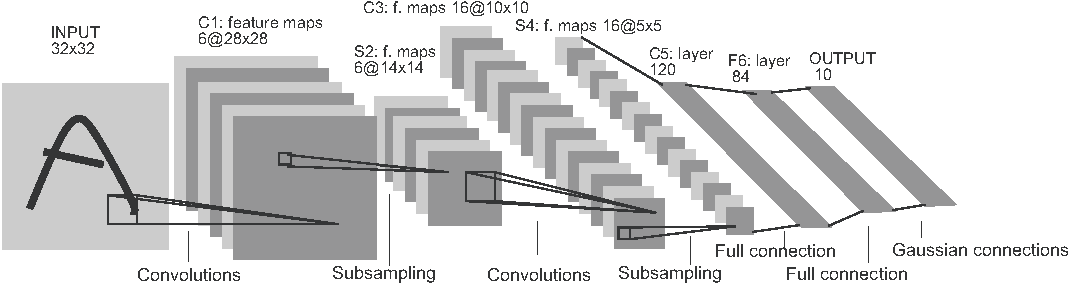
\includegraphics[width=12cm]{img/ch03/LeNet5.pdf}
\captionof{figure}[Architecture of LeNet5]{Architecture of LeNet5 that set a pattern for modern \acp{CNN} \cite{Lecun98gradient-basedlearning}}
\label{fig:lenet5}
\end{center}

\subsection{Data Augmentation}
In summary it can be stated that \ac{conv} layers are trained to detect features and \ac{fc} layers are trained to detect relations between features that indicate specific classifiers. To achieve this, \acp{CNN} need to be trained with datasets specific to their application that must be of good quality \cite{Schweitzer2017}. Factors contributing to the quality of datasets are the quality of their images (e.g. high resolution, little noise) and labels (e.g. number of classes, general presence of regions associated with labels). However large sets of such data may be hard to come by due to scarce availability (e.g. of datasets for highly specialized applications) or the amount of effort creating those takes. Lastly, they may simply cost a lot of time to produce.\\
\emph{Data Augmentation} promises to solve this problem by altering datasets through application of various operations: for instance images can be stretched, mirrored, zoomed and rotated or color filters can be applied to them. As long as these changes are transferred to the labels of images, these altered datasets drastically increase the size of datasets that can be used for training \acp{CNN}. This can also potentially help to make detections more reliable for special cases: as an example, datasets that feature cars would mostly show cars in their surroundings, hence they would rarely be cut off in images. Altering images so they cut off parts of cars like wheels may enable \acp{CNN} to recognize cars without requiring cars to actually show wheels on images.
\clearpage

\section{Transforms}
\label{ch03-transforms}
In computer graphics, objects in 3D space are organized in a \emph{scene graph} where nodes use \emph{transforms} to express their location, rotation and scale relative to their parent node. Those attributes can be expressed in vectors with three elements each, where each of these elements represents the effect of a transformation for one axis. A complete transformation with a location $l$, rotation $r$ and scale $s$ for an object could be written as:
\begin{equation}
    l = \begin{pmatrix} 0\\0\\0\end{pmatrix}, r = \begin{pmatrix} 0\\90\\0\end{pmatrix},  s = \begin{pmatrix} 1\\1\\1\end{pmatrix}
\end{equation}
This describes an object that is located at the center of the coordinate system, is rotated around the $y$ axis by $90$ degrees and has the default scale of $1$ applied to all axis.
\subsubsection{Operations on Transforms}
Several operations can be performed on transforms, including translation, scaling and rotating. Those operations can be chained using transformation matrices that the following paragraphs will illustrate. These transformation matrices use homogeneous coordinates as their use of higher dimensions to perform additive operations using multiplication. \cite{10.1007/978-1-4471-6290-2}
\paragraph{Translation} A vector $l$ can be translated by an offset $o$ to a new location $l_n$ can be written as an addition of two vectors
\begin{equation}
    l' = l + o = \begin{pmatrix}l_{1} + o_1\\l_{2}+ o_{2}\\l_{3} + o_{3}\end{pmatrix}
\end{equation}
or using a matrix $m_t$
\begin{equation}
    l' = m_t \times l =\begin{pmatrix}
        1 & 0 & 0 & o_1\\
        0 & 1 & 0 & o_2\\
        0 & 0 & 1 & o_3\\
        0 & 0 & 0 & 1
    \end{pmatrix} \times  \begin{pmatrix}l_1 \\ l_2 \\ l_3 \\ 1\end{pmatrix}
    \label{eq:matrix-translate}
\end{equation}
\paragraph{Scaling} A vector $s$ is scaled by axis-specific scalars $o$ that result in a new scale $s_n$ can be expressed using a matrix $m_s$
\begin{equation}
    s' = m_s \times s = \begin{pmatrix}
        o_1 & 0 & 0 & 0\\
        0 & o_2 & 0 & 0\\
        0 & 0 & o_3 & 0\\
        0 & 0 & 0 & 1
    \end{pmatrix} \times \begin{pmatrix}s_1 \\ s_2 \\ s_3 \\ 1\end{pmatrix}
    \label{eq:matrix-scale}
\end{equation}
\paragraph{Rotation} Rotating vectors involves the use of trigonometric functions and can be done per axis using a separate matrix. For rotating a vector $v$ around the $x$ axis by $\alpha$ degrees, matrix $m_{rx}$ is used:
\begin{equation}
    v' = m_{rx} \times v = \begin{pmatrix}
        1 & 0 & 0 &  0\\
        0 & \cos{\alpha} & -\sin{\alpha} & 0\\
        0 & \sin{\alpha} & \cos{\alpha} & 0\\
        0 & 0 & 0 & 1
    \end{pmatrix} \times \begin{pmatrix}v_1 \\ v_2 \\ v_3 \\ 1\end{pmatrix}
\end{equation}
To rotate a vector $v$ around the $y$ axis by $\beta$ degrees, matrix $m_{ry}$ is used:
\begin{equation}
    v' = m_{ry} \times v = \begin{pmatrix}
        \cos{\beta} & 0 & \sin{\beta} &  0\\
        0 & 1 & 0 & 0\\
        -\sin{\beta} & 0 & \cos{\beta} & 0\\
        0 & 0 & 0 & 1
    \end{pmatrix} \times \begin{pmatrix}v_1 \\ v_2 \\ v_3 \\ 1\end{pmatrix}
\end{equation}
Subsequently, a vector $v$ can be rotated around the $z$ axis by $\gamma$ degrees by using matrix $m_{rz}$:
\begin{equation}
    v' = m_{rz} \times v = \begin{pmatrix}
        \cos{\gamma} & -\sin{\gamma} & 0 & 0\\
        \sin{\gamma} & \cos{\gamma} & 0 & 0\\
        0 & 0 & 1 & 0\\
        0 & 0 & 0 & 1
    \end{pmatrix} \times \begin{pmatrix}v_1 \\ v_2 \\ v_3 \\ 1\end{pmatrix}
\end{equation}
One can also rotate a vector $v$ around the $x$, $y$ and $z$ axis by $\alpha$, $\beta$ and $\gamma$ respectively by multiplying the abovementioned matrices $m_{rx}$, $m_{ry}$ and $m_{rz}$:% (where $c(x)$ is $\cos{x}$ and $s(x)$ is $\sin{x}$):
\begin{equation}
    %\begin{split}
    v' = m_{rx} \times m_{ry} \times m_{rz} \times v%\\
    %v' & = m_{rx} \times m_{ry} \times m_{rz} \times v%\\
     %& = \begin{pmatrix}
        %\cos{\beta}\cos{\gamma} & \cos{\beta}\sin{\gamma} & -\sin{\beta} & 0\\
        %\sin{\alpha}\sin{\beta}\cos{\gamma}-\cos{\alpha}\sin{\gamma} & \sin{\alpha}\sin{\beta}\sin{\gamma}+\cos{\alpha}\cos{\gamma} & \sin{\alpha}\cos{\beta} & 0 \\
        %\cos{\alpha}\sin{\beta}\cos{\gamma}+\sin{\alpha}\sin{\gamma} & \cos{\alpha}\sin{\beta}\sin{\gamma}-\sin{\alpha}\cos{\gamma} & \cos{\alpha}\cos{\beta} & 0\\
        %c(\beta)c(\gamma) & c(\beta)s(\gamma) & -s(\beta) & 0\\
        %s(\alpha)s(\beta)c(\gamma)-c(\alpha)s(\gamma) & s(\alpha)s(\beta)s(\gamma)+c(\alpha)c(\gamma) & s(\alpha)c(\beta) & 0 \\
        %c(\alpha)s(\beta)c(\gamma)+s(\alpha)s(\gamma) & c(\alpha)s(\beta)s(\gamma)-s(\alpha)c(\gamma) & c(\alpha)c(\beta) & 0\\
        %0 & 0 & 0 & 1
    %\end{pmatrix} \times \begin{pmatrix}v_1 \\ v_2 \\ v_3 \\ 1\end{pmatrix}
    %\end{split}
    \label{eq:matrix-rotate}
\end{equation}

\subsubsection{Combining Operations}
To combine operations on a vector $v$ one can chain the transformation matrices shown in the equations \ref{eq:matrix-translate}, \ref{eq:matrix-scale} and \ref{eq:matrix-rotate}. Matrix multiplication is not commutative though, therefore the order the matrices are multiplied in matters: rotating a vector and translating it afterwards is not equivalent to first translating a vector and then rotating the vector. Equation \ref{eq:matrix-combined} shows how these matrices can be combined. In this example, the vector is first rotated, then translated and lastly it is scaled.
\begin{equation}
    v' = m_s \times m_t \times m_r \times v
    \label{eq:matrix-combined}
\end{equation}
As objects' transforms only hold information about translation, scaling and rotation relative to their frame of reference, which usually is their parent object, the absolute transform of an object in world space can be calculated by chaining all transformation matrices of its parents. This information may be needed in game logic and is needed in rendering.

\subsubsection{Projection to 2D Space}
\ref{eq:projection-matrix} describes a projection matrix $m_{proj}$ and a transformation matrix $m_{tra}$ applied to a vector $v$. While $m_{proj}$ projects a vector according to the camera's field-of-view $\phi$ and clipping planes $Z$, multiplication with $m_{tra}$ maps the projected vector to a 2D plane considering the size of the plane $d$ in pixels, the size of the clipping area $c$ and the offset of the clipping area to the plane $o$ in pixels \cite{Seufert2009}. The $z$ component of $v'$ will indicate whether $v$ was behind the camera or in front of it.
\begin{equation}
    \begin{split}
    m_{proj} & = \begin{pmatrix}
        \cot{\frac{\phi_h}{2}} & 0 & 0 & 0\\
        0 & \cot{\frac{\phi_v}{2}} & 0 & 0\\
        0 & 0 & \frac{Z_h}{Z_h-Z_v} & 1\\
        0 & 0 & \frac{-Z_h Z_v}{Z_h-Z_v} & 0
    \end{pmatrix}\\ 
    m_{tra} & = \begin{pmatrix}
        \frac{d_b}{c_b} & 0 & 0 & 0\\
        0 & -\frac{d_h}{c_h} & 0 & 0\\
        0 & 0 & 1 & 0\\
        -\frac{o_hd_b}{c_b} & \frac{o_v d_h}{c_h} & 0 & 1
    \end{pmatrix}\\
    v' & = m_{proj} \times m_{tra} \times v
    \end{split}
    \label{eq:projection-matrix}
\end{equation}
\clearpage

\section{3D Graphics}
This section provides a brief overview about the structure and looks of 3D models, different rendering techniques and selected post-processing effects.
\subsection{Models}
\subsubsection{Meshes}
\emph{Meshes} define the geometry of 3D models and are made of \emph{Vertices}, which are data-structures that hold information about points in 3D space. Depending on the application, vertices can hold additional information, e.g. color and reflectance. Vertices can be connected to each other via \emph{edges}. Multiple edges can be combined to create \emph{faces}. These are planar surfaces defined by a set of usually three (called \emph{polygon}) or four (called \emph{quad}) edges. Vectors that are perpendicular to faces are called \emph{normals} and are often used in rendering, for instance to calculate light-reflections on surfaces. A \emph{mesh} is an individual set of vertices, edges and faces.\\
Figure \ref{fig:3d-mesh-construction} shows an initial set of three individual vertices (\ref{fig:3d-vertices}) that are connected via edges (\ref{fig:3d-edges}), then combined to a face (\ref{fig:3d-face}) and eventually used as part of a complex mesh (\ref{fig:3d-mesh}).

\newlength{\twosubht}
\newsavebox{\twosubbox}

\begin{figure}[htp]
    \sbox\twosubbox{%
      \resizebox{\dimexpr.9\textwidth-1em}{!}{%
        
\includegraphics[height=3cm]{img/ch03/Basics01_Vertices.png}
        
\includegraphics[height=3cm]{img/ch03/Basics01_Vertices.png}
        
\includegraphics[height=3cm]{img/ch03/Basics01_Vertices.png}
        
\includegraphics[height=3cm]{img/ch03/Basics01_Vertices.png}
      }%
    }
    \setlength{\twosubht}{\ht\twosubbox}
    % typeset
    \centering
    \subcaptionbox{\label{fig:3d-vertices}}{%
        
\includegraphics[height=\twosubht]{img/ch03/Basics01_Vertices.png}
    }\quad
    \subcaptionbox{\label{fig:3d-edges}}{%
        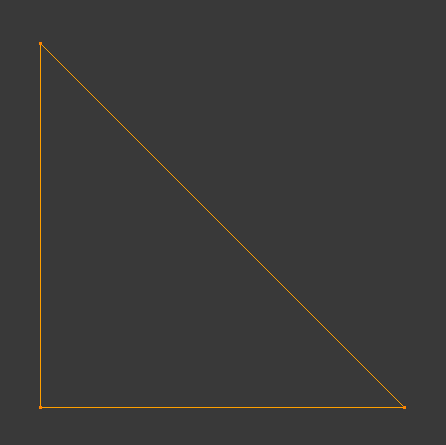
\includegraphics[height=\twosubht]{img/ch03/Basics02_Edges.png}
    }\quad
    \subcaptionbox{\label{fig:3d-face}}{%
        
\includegraphics[height=\twosubht]{img/ch03/Basics03_Faces.png}
    }\quad
    \subcaptionbox{\label{fig:3d-mesh}}{%
        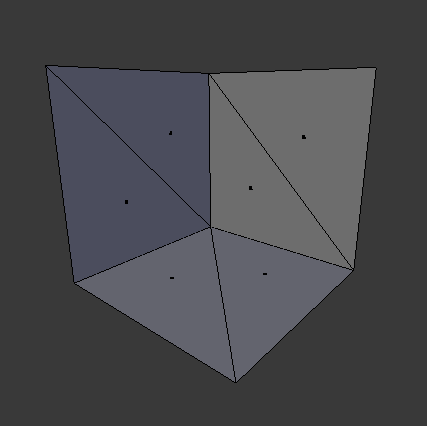
\includegraphics[height=\twosubht]{img/ch03/Basics04_Meshes.png}
    }
    \caption{Construction of a mesh}
    \label{fig:3d-mesh-construction}
\end{figure}

\subsubsection{Materials}
\label{ch03-materials}
\emph{Materials} describe how faces of meshes shall be rendered. They can define properties that are either dependent or independent of the location or size of a surface. Properties that are independent of the location and size of surfaces are often limited to primitive simple features such as color and reflectance.\\
In order to enable more powerful effects, materials need to be able to map each point on a surface of a mesh to a texture coordinate. This process is called UV mapping and it provides a way to "wrap" textures around meshes by defining a 2D coordinate on a texture (using $u$ and $v$ values for width and height in an interval of $[0, 1]$) for each vertex of a mesh \cite{BlenderUVEditor}. Once this map exists, materials can use \emph{texture mapping} to add various effects to a mesh's surface, including:
\begin{description}
    \item[Texture] A \emph{texture} is an image that is wrapped around a mesh so its surfaces show parts of it. They can be used to add great visual detail to meshes that would not be feasible to implement with geometry alone.
    \item[Normal Map] \emph{Normal maps} add geometric visual detail to rendered surfaces by lighting bumps that are not present in the mesh \cite{UnityDocNormalmap}.  This information is calculated from the normals of faces of high-resolution meshes and can then be mapped to low-resolution meshes \cite{Cohen:1998:AS:280814.280832}\cite{745285}. They effectively allow to preserve the visual level of detail of high-resolution meshes while low-resolution meshes are used to save resources in the rendering process.
    \item[Height Map] \emph{Height maps} are similar to normal maps in that they add visual detail geometric visual to surfaces that are not present in the mesh. However they  manipulate the visible area of the surface texture so that individual parts of the surface occlude others and thus give an impression of depth to the surface.
    \item[Specular Map] \emph{Specular maps} are used to control the amount of specular reflectivity of individual parts of surfaces \cite{UnityDocSpecularmap}. This effect is often used to imitate metallic surfaces and requires some form of environment map that can be used to reflect parts of the environment on the surface.
\end{description}
Figure \ref{fig:3d-cube-uv-mapping} shows the UV-map of a cube and a texture laid over it. The texture is wrapped around the cube so that each side shows a number contained within the texture.

\begin{center}
%\begin{figure}[t]
%\centering
    \noindent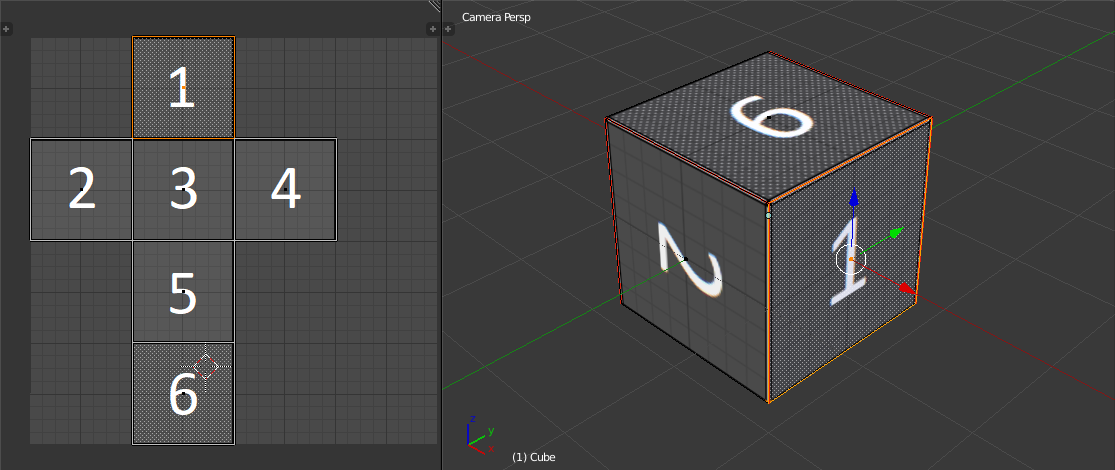
\includegraphics[width=12cm]{img/ch03/CubeUVMapping.png}
    \captionof{figure}[UV-map of a cube]{UV-map of a cube on top of a texture}
    \label{fig:3d-cube-uv-mapping}
%\end{figure}
\end{center}

\subsection{Rendering}
The process of creating images of 3D models or scenes is called \emph{Rendering}. It draws objects contained in scenes from the viewpoint of a virtual camera to a 2D plane and takes materials and lighting information into account. There are two categories of renderers: \emph{offline renderers} usually strive for realistic visual output and use expensive techniques to create images, such as physics-based rendering. The drawbacks of those is that the time they require to render scenes is directly dependent on the scene's complexity. \emph{Online renderers} run in real-time to produce images in quick succession.\\
If these images are generated and shown just quickly enough, movements in the scene appear continuous: in studies, the majority of participants could distinguish modulated light (such as displays) at rates of $50-90 Hz$, however other studies found that this number may be as high as $500 Hz$ \cite{Davis2015}. While there is a scientific disagreement about the rate of images that humans are able to perceive, process and distinguish, the industry introduced standards for electronic displays. Modern displays present images at $60-144 Hz$.\\
The following sections will show two technologies widely used in offline and online renderers.

\subsubsection{Raytracing}
A widely used technology used in offline renderers is \emph{raytracing}. To a certain extend, it imitates real cameras in that for each pixel in the image that is to be rendered, it sends rays from a virtual camera to objects in the scene to calculate the color at the point where it hit an object, considering the material of the surface that was hit. Reflective properties of materials are taken into account by sending rays from the point an object was hit at. Noise and strong contrasts between pixels in the image can be countered by casting multiple rays per pixel and averaging the resulting color.\\
Raytracing is used in software like \emph{Blender} that aims to produce physically correct output.

\subsubsection{Rasterization} Modern games use \emph{rasterization} to render scenes to the screen. This approach processes 3D objects through various stages that differ in their exact implementation but share the same concepts. First, geometry is processed by a \emph{vertex shader} that transforms all vertices of the geometry to screen space (using the transformations shown in \ref{ch03-transforms}). This shader may manipulate properties like color of vertices but it can not create new geometry. The geometry is further passed to a \emph{geometry shader} which, contrary to vertex shaders, may add to the geometry to add detail to it. For instance, it may make use of technologies like tessellation which sub-divides geometry into further triangles to round the silhouette of geometry. The resulting geometry is broken down into \emph{fragments} by discarding vertices that are not visible in the image because they are either not in the field-of-view of the camera (\emph{clipping}) or are not facing the camera (\emph{culling}).
Then the geometry is rasterized: polygons are translated to individual pixels in the \emph{frame buffer}. By performing a so called \emph{depth test} for each pixel, only the geometry that is nearest to the camera will be drawn for an individual pixel.
Lastly, resulting the pixels are passed through a \emph{pixel shader} that may implement various effects of texture maps described in \ref{ch03-materials} such as normal maps and specular maps. They may also manipulate the \emph{z-buffer} that is used to store depth information. When at later stages textures are passed to pixel shaders, they may manipulate the textures by applying two-dimensional effects like blur.\\
\emph{Post-processing} is often done in vertex and pixel shaders and allows to apply effects to the scene that require information about the entire image, such as \emph{anti-aliasing} (used to smooth out hard edges), \emph{bloom} (glow of light seen in real cameras) and blur (e.g. \emph{motion blur} and blur caused by depth in images that is out of focus, \emph{depth of field}).
\clearpage

% //////////////////////////////////////////////////
\section{Game Engines}
Game engines are software environments that provide a set of components that allows to create and run video games. They feature a \emph{rendering} and \emph{audio engine} used for audio and visual output and a \emph{physics engine} to simulate aspects of physics such as gravity and collision. Most feature a so called \emph{game loop} that orchestrates these engines and processes a game's logic (shown in Figure \ref{fig:game-loop}). One cycle of this loop is commonly referred to as a \emph{frame}. Depending on the implementation of the game loop, a game may enter an idle state after rendering to limit the amount of \ac{FPS} or update the scene multiple times per frame at times when updates are required in rapid succession. It may also skip rendering when rendering takes too long and updates need to be processed (\emph{frame skipping}).

\begin{figure}[t]
    \centering
    \noindent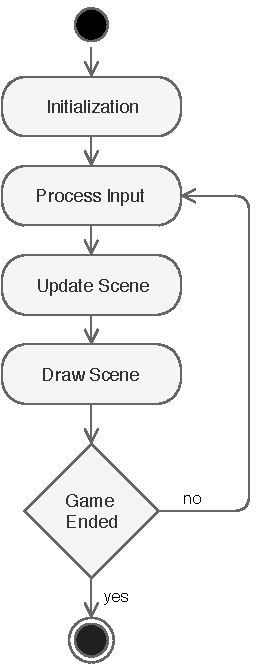
\includegraphics[width=4cm]{img/ch03/GameLoop_05.pdf}
    \captionof{figure}{A simple game loop}
    \label{fig:game-loop}
\end{figure}

\subsection{Development Tools}
The tools used in the development process of games is heavily dependent on the game engine that was used. While some feature a set of command-line tools to pack resources, build folder structures and compile binary executable files, others combine all of these features into one software-suite. \emph{World building} is an essential task in game development and also differs greatly in implementation across game engines: the \emph{Source Engine} (powering \emph{"Half-Life 2"} by \emph{Valve}) requires level designers to use an editor to create scenes (\emph{maps}) and compile them into a proprietary format which is then parsed by the engine at run-time \cite{SourceHammerEditor}. Others, like the \emph{Unreal Engine} (powering \emph{"Life is Strange"} by \emph{Dontnod Entertainment}) and the \emph{Unity Engine} (powering \emph{"Ghost of a Tale"} by \emph{Lionel Gallat}) feature all-in-one editors that combine management of assets and world building \cite{UnrealLevelEditor}\cite{UnityDocsOverview}.

\subsection{Adding Logic to a Game}
While game engines handle sophisticated tasks like rendering and simulating physics on their own, logic is implemented by game developers. There are different ways to add logic to games and this section will focus on two approaches that are widely used.

\subsubsection{Object Oriented Programming}
A traditional approach to enriching entities in scenes with logic is \emph{\ac{OOP}}. In this approach, entities inherit from a base class that holds basic information (e.g. the entity's transform and name) and provides functions used by the engine and other classes that may be overridden (e.g. methods to draw or update the entity). This approach usually works fine for high-level components that manage entities or scenes, however it often involves inheriting multiple classes and when used at a lower level (e.g. on single entities), this results in very complex classes. In scenarios where multiple inheritance is not possible (due to programming language limitations), interfaces may be used. However implementing interfaces multiple times leads to code duplication. Also, behaviours and functionalities are fixed parts of implementations.

\subsubsection{Entity-Component-System}
A common solution to the problems introduced by inheritance in \ac{OOP} is to shift the implementation of interfaces to other classes and make use of composition. \emph{\acp{ECS}} aim to shift the focus from entities as programmable units towards isolated components that represent behaviours. Following the emph{single responsibility principle}, each component is meant to serve and implement a single use. This results in high re-usability of components and reduces code duplication. In \acp{ECS}, entities usually hold a list of components and hence, contrary to \ac{OOP}, entities may have components added to or removed from them at run-time. 
\chapter{Conceptual Design}
\label{chap:conceptual-design}
The goal of this thesis is to develop a system that allows generating large sets of images for training neural networks. As this environment shall be used as a drop-in replacement for conventional methods such as taking photos and labelling those by hand, the generated images must be of excellent quality and labelled.\\
This chapter will introduce the terminology, central ideas and architectural basics of a concept that can be used to implement the system by explaining its high-level features using use-cases, refining those to specific user-interactions and deducing components from those. 

%////////////////////////////////////////////////
\section{System Environment and Terminology}
% *** Scenes
The system features at least one virtual 3D environment (a \emph{scene}) that represents a specific place (either an existing or non-existing place) and a virtual \emph{robot} that operates in said environment. It is used by two groups of users: \emph{designers} and \emph{\ac{AI} engineers}. Figure \ref{fig:use-cases-abstract} shows these groups of users and their high-level and abstract use-cases.
\begin{figure}[t]
    \centering
    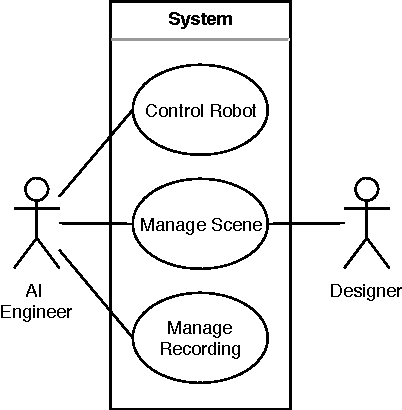
\includegraphics[width=6cm]{img/ch04/UseCases_HighLevel.pdf}
    \captionof{figure}{High-level Use-Cases}
    \label{fig:use-cases-abstract}
\end{figure}
% *** Robots
A \emph{virtual robot} is a representation of a real or fictional robot. It is mainly used to navigate a virtual camera used for capturing \emph{records} from the robot's perspective while its movement is restricted by its body's specifics, considering different types of drives (such as limbs or wheels) and their respective attributes (such as degrees of freedom or torque).\\
% *** Designers
Scenes need to be created, modeled using geometry, populated with entities and configured. \emph{Designers} set up scenes so that they can be used by \acs{AI} engineers in a production environment. They recreate existing or non-existing places by adding 3D objects and \emph{entities} to scenes. Depending on the specific use of the scene and individual objects in it, designers can add \emph{mutators} to any entities in a scene and equip them with an initial configuration. They can also add waypoints to scenes that constitute paths for robots to travel along.\\
% *** Records
A \emph{record} is a data-structure that contains an image and a list of labels. \emph{Labels} hold information about the region in an image that a classifier was identified at. Records may contain meta-data about images, such as the location and view-angles of the camera at the time of capturing the images. This meta-data may prove useful when reconstructing the exact position of robots from generated sets of images. The types asterisked in Figure \ref{fig:classes-record} are placeholders that are implementation-specific.
\begin{figure}[b]
    \centering
    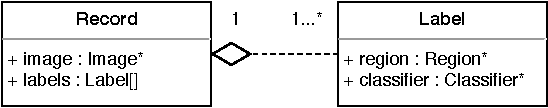
\includegraphics[width=8cm]{img/ch04/Classes_Record.pdf}
    \captionof{figure}{Data-structure "Record"}
    \label{fig:classes-record}
\end{figure}
% *** Entities
\emph{Entities} can be understood as objects in scenes that add more content to a scene than just geometry. Any objects that interact with scenes or other objects within scenes can be understood as entities. This includes light-sources and objects that can be interacted with physically (like doors).
% *** AI engineers
\emph{\acs{AI} engineers} use the system to capture records. To do so they can use the system in one of two modes: \emph{"manual control"} lets them take control of robots and maneuver them in scenes, \emph{"automatic mode"} allows them to let robots travel along preconfigured paths. At any time they can toggle automatic capture and labelling of images and activity of mutators.\\
% *** Mutators
In order to provide visual variety to the generated images, \emph{mutators} alter the state of various attributes of entities in scenes in a step-wise fashion. For instance, they can be used to manipulate the intensity, range and color of light-sources, resulting in images that feature different lighting. The amount of steps a mutator needs to perform alterations on before completing a full mutation-cycle depends on the range of values it can assign to attributes. Binary mutators (e.g. used to turn lights on or off) only take two steps to complete a mutation-cycle, more complex mutators may step through arbitrary value ranges though (e.g. dimming light-intensity from 100 to 0 percent in 5 percent steps, requiring 20 steps total). \\
% *** Waypoints
\emph{Waypoints} (shown in \ref{fig:classes-waypoint}) are simple coordinates in the 3D space of a scene that can be used to define paths that robots can travel along. They may hold a reference to another waypoint, allowing designers and \acs{AI} engineers to easily create paths.  
\begin{figure}[t]
    \centering
    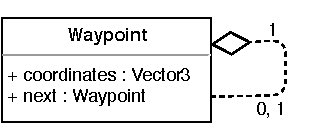
\includegraphics[width=4cm]{img/ch04/Classes_Waypoint.pdf}
    \captionof{figure}{Data-structure "Waypoint"}
    \label{fig:classes-waypoint}
\end{figure}
The specific design of scenes and robots and the implementation of mutators depend on the scenario that the object-recognition software, that is to be trained, is used in: software run on cars should be trained using images generated in scenes that represent the environment the car is planned to be operated in and the robots used in these scenes should be modeled so they closely represent the car the software is to be run on, considering physical attributes (such as the car's shape, surfaces and size), behaviour (including acceleration, weight and steering)  and sensor-placement, where visual sensors such as cameras are of the highest importance to the process of generating images.

%\begin{center}
%\noindent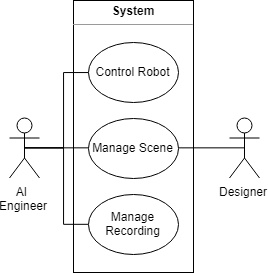
\includegraphics[width=6cm]{img/ch04/Use_Cases_06.png}
%\captionof{figure}{Abstract use-Cases}
%\label{fig:use-cases-abstract}
%\end{center}

%////////////////////////////////////////////////
\section{User Interaction}
The use-cases shown in Figure \ref{fig:use-cases-abstract} need to be further refined into specific features before specific components can be deduced from them.

\subsubsection{Use-Case "Control Robot"}
\acs{AI} engineers may want to take control of robots and maneuver them in scenes by accelerating, decelerating and steering or resetting them in case of being unable to maneuver. This may be the case when the robot was flipped or trapped between objects. Operating in manual mode can also be used to evaluate the usefulness (e.g. mobility) of certain robot-bodies in certain environments, presuming that the scene and robot behave like they would in real-life, and may even be used to validate that the specific combination of robot-body and scene in a scenario operates as expected. This may require physics simulation for gravity and collision detection, and mechanics simulation for kinematics.\\
Also, manual control of robots requires a careful choice of input-devices: \acs{AI} engineers should use input-devices that allow for precise and true to original control of robots. For instance, a combination of a steering wheel and gas and break pedals closely resembles the control options present in cars whereas two independent joysticks can be used to control torque of two continuous tracks on tracked vehicles.

\subsubsection{Use-Case "Manage Recording"}
\acs{AI} engineers need to be able to start and stop automatic capturing of records. As records are effectively pairs of images and a list of labels, both elements of these pairs must be provided by the system: it needs to feature a component that captures images from a camera held by a robot in a scene. To populate records with labels the system needs to provide a component that identifies classifiers in the captured images.

\subsubsection{Use-Case "Manage Scene"}
Designers need to import assets (such as 3D models, materials and textures) into the system in order to add geometry to scenes and configure robots that can be used by \acs{AI} engineers. Depending on the requirements of the scenario at hand, designers may need to add various entities such as light-sources or movable objects to scenes and equip them with an initial set of configurable mutators. Optionally, designers may add waypoints to scenes to provide paths for robots to travel along.\\
\acs{AI} engineers may want to configure mutators at run-time in order to explore and study their effects on scenes (such as changes in lighting). Also they may want to add or change waypoints to vary what part of a scene is captured during recording sessions.

Figure \ref{fig:use-cases} summarizes these refinements and shows that most use-cases are interacted with by only one role, separating them into groups of use-cases required for initial setup ("Create ..."), run-time ("Robot" and "Recording" use-cases) and a special group that is used to tweak run-time behaviour to achieve varying sets of records ("Manage Waypoints", "Manage Mutators"). 
\begin{figure}
    \centering
    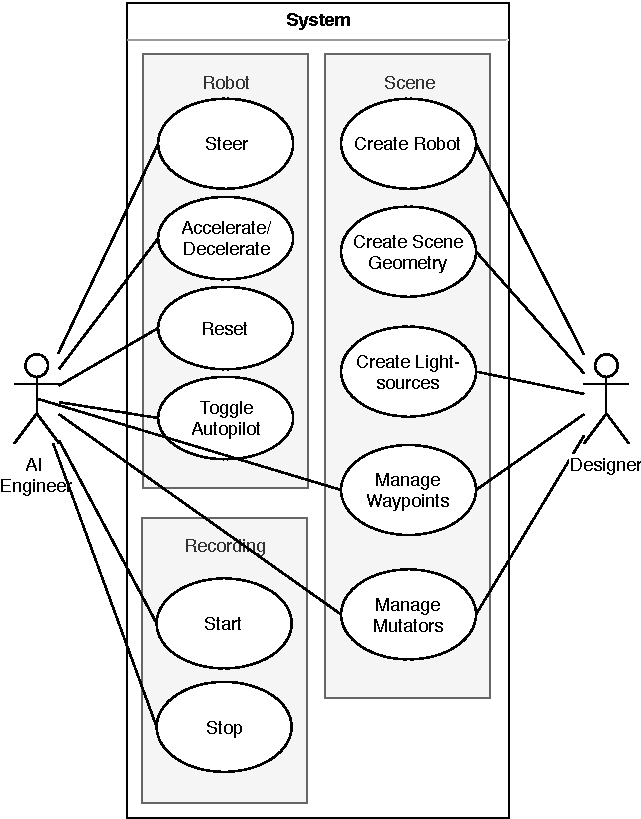
\includegraphics[width=10cm]{img/ch04/UseCases_Fine.pdf}
    \captionof{figure}{Refined Use-Cases}
    \label{fig:use-cases}
\end{figure}
\clearpage

%////////////////////////////////////////////////
\section{Automatic Mode: Control Flow}
\label{ch04-control-flow}
The abovementioned automatic mode the system can run in (shown in Figure \ref{fig:control-flow}) is used to automate the process of moving robots in scenes, capturing records and mutating scenes.\\
When active, it will alter a scene by advancing mutation and capture records as long as the mutation-cycle has not been completed. Once the mutation-cycle is completed, the mutation will be reset. If the robot in the scene has not reached its destination yet it will be moved and the process continues by running the mutation-cycle again.\\
\begin{figure}[htb!]
    \centering
    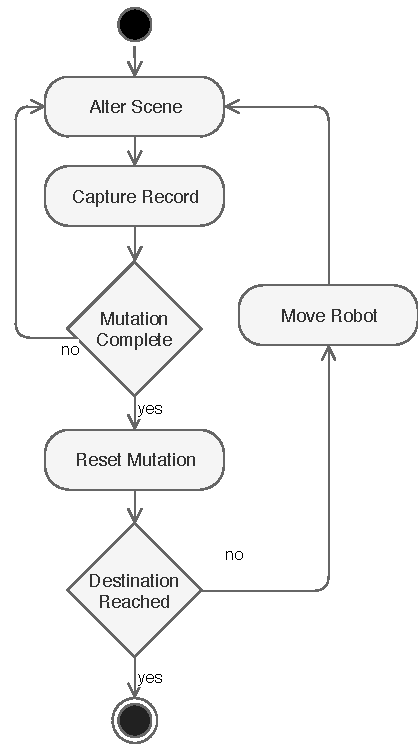
\includegraphics[width=8cm]{img/ch04/ActivityDiagram_HighLevel.pdf}
    \captionof{figure}{Control flow of the automatic mode}
    \label{fig:control-flow}
\end{figure}
This behaviour effectively iterates through all mutations set up for a scene, applies them, captures records for each mutation and does so each time the robots is moved. The only step that is largely independent of implementation is "Reset Mutation" as it will only recover the initial state of all entities in a scene. "Alter Scene", "Capture Record" and "Move Robot" are heavily dependent on the scenario at hand and the specific implementation. For instance, "Move Robot" may either simulate movement of robots by using their physical properties and bodies or simply move them to another position instantly.

%////////////////////////////////////////////////
\section{Components}
While the high-level use-cases (Figure \ref{fig:use-cases-abstract}) implicate the need for three high-level components, refinement of the use-cases (Figure \ref{fig:use-cases}) encourages the use of packages to encapsulate complex components. Figure \ref{fig:component-diagram} shows an abstract component used for controlling robots (\emph{RobotController}), a package that provides components needed for capturing records (\emph{Recording}) and another one that contains components used to manage scenes (\emph{SceneManagement}).
\begin{figure}[hb!]
    \centering
    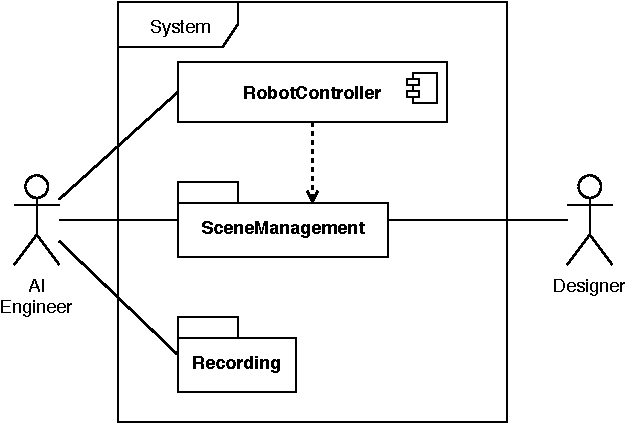
\includegraphics[width=10cm]{img/ch04/ComponentDiagram_System02.pdf}
    \captionof{figure}{High-level component diagram}
    \label{fig:component-diagram}
\end{figure}
% Recording
The "Recording"-package (Figure \ref{fig:component-diagram-recording}) contains two abstract components: \emph{CaptureController} is used to start and stop automatic capturing of records. It captures images and enriches those with labels by making use of the \emph{ImageLabeller}-component. The ImageLabeller-component needs to be able to identify classifiers in images. As neither capturing images nor identifying classifiers are necessarily trivial tasks, the implementation of both components is greatly influenced and in some cases dictated by the scenario and technology used. While capturing images is usually easily achieved in software that features visualization of the virtual environments, "headless" software running without any visual output may require external software to render images resulting in the CaptureController-component effectively being implemented by software running on two separate systems, increasing the complexity of the implementation.
\begin{figure}
    \centering
    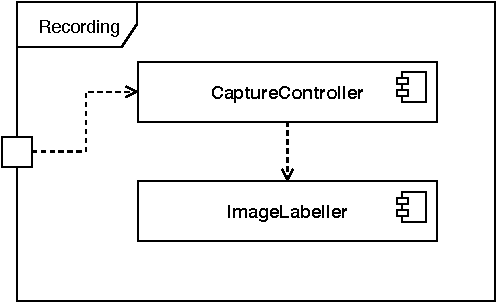
\includegraphics[width=8cm]{img/ch04/ComponentDiagram_Recording.pdf}
    \captionof{figure}{"Recording"-package}
    \label{fig:component-diagram-recording}
\end{figure}
% Scenemanagement
As indicated by the use-cases involved in interacting with scenes (Figure \ref{fig:use-cases}), the "SceneManagement"-package (Figure \ref{fig:component-diagram-scenemanagement}) features multiple components.\\
The \emph{SceneGeometry}-component holds all 3D objects of a scene that amount to the visual representation and physical bodies of the place the scene is meant to represent. This includes both, objects that feature or lack actual physical collision (e.g. clouds).\\
A \emph{SceneEntities}-component stores all entities of a scene and manages their life-cycles. In a simple implementation this component could use lists or arrays internally.
\begin{figure}[hb!]
    \centering
    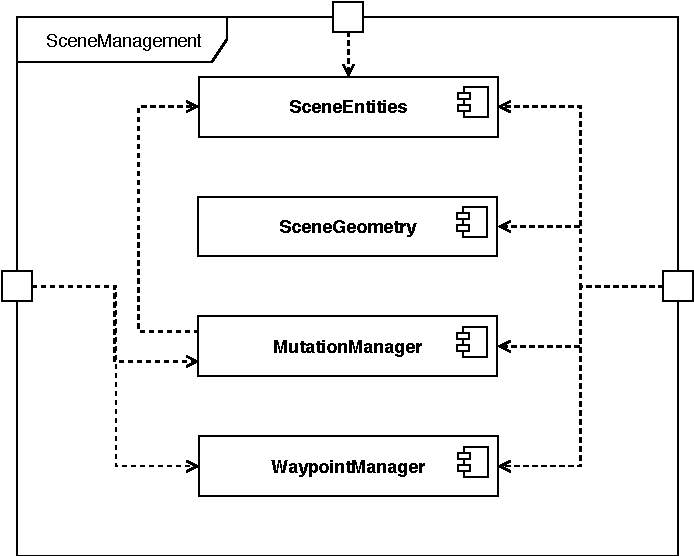
\includegraphics[width=11cm]{img/ch04/ComponentDiagram_SceneManagement.pdf}
    \captionof{figure}{"SceneManagement"-package}
    \label{fig:component-diagram-scenemanagement}
\end{figure}
In each scene there is one \emph{MutationManager}-component. It holds a list of all mutators in a scene and, when active, advances only one mutator in a scene at a time so that each possible combination of attribute-mutations is present in a scene at least once. This implicates that each additional mutator added to a scene multiplies the number of steps required to fully step through all attribute-mutations by the number of steps required to step through the new mutator; the number of mutation-steps required to complete a full mutation-cycle grows exponentially.\\
The MutationManager-component also provides a reset-feature that resets all attribute-mutations to a defined initial state.
The \emph{WaypointManager}-component holds a list of waypoints where each waypoint constitutes a path by chaining references to other waypoints. Its purpose is to provide an overview of paths configured in scenes.
%
%\section{Summary}
%This concept is designed so that it is operating-system-, platform- and framework-agnostic. This results in an abstract concept that describes a basic architecture and abstract components and allows for flexibility in implementations: components may be implemented and run on the same or many separate machines, which is of particular interest for research-facilities that operate large clusters of computers.
\chapter{Implementation Using Game Engines as Renderers and Frontends}
\label{chap:implementations}
In this chapter the concept presented in \ref{chap:conceptual-design} will be implemented using a game engine as renderer and frontend. After a brief overview of the goals and constraints of this specific implementation, it will look into reasons why games engines are suited for implementing the concept and how one was chosen for this implementation. Analogue to the steps described in the concept, this chapter will show how an existing environment was reconstructed to be used as a scene and how a robot was imported into this scene and optimized to work in the game engine. Further, it will show how mutators were implemented and used in the scene and compare different approaches to identifying objects. Lastly, this chapter shows how records were saved and how this implementation performed during recording sessions.

%////////////////////////////////////////////////
\section{Goals and Constraints of the Implementation}
\label{section:goals-and-constraints}
Inspired by a thesis written by Schweitzer in 2017 that approached using \acsp{CNN} that detect doors on autonomous robots \cite{Schweitzer2017}, the goal of this thesis' implementation became to generate records that could be used to train \acsp{CNN} that detect doors.\\ 
The environment chosen for this implementation was the second floor of building "A" of University of Applied Sciences Mannheim as this building houses the Faculty of Computer Science and the Institute of Robotics is located in the second floor.\\
This implementation of the concept had the working title \emph{\ac{VERE}}. While it produced records that could be used to train \acsp{CNN}, no such tests were performed due to time-constraints.

\section{Using Game Engines}
The decision to use game engines to implement the concept was based on the observation that video games have always striven after improved visual presentation and more intuitive user interaction in order to attract customers, leading to the general availability of game engines that feature impressive graphical detail (as demonstrated in figure \ref{fig:unity-demo-graphics}), intuitive methods to interact with users and great performance on modern computer systems. Their ability to produce realistic images in real-time made them an attractive alternative to traditional offline renderers.
\begin{center}
\noindent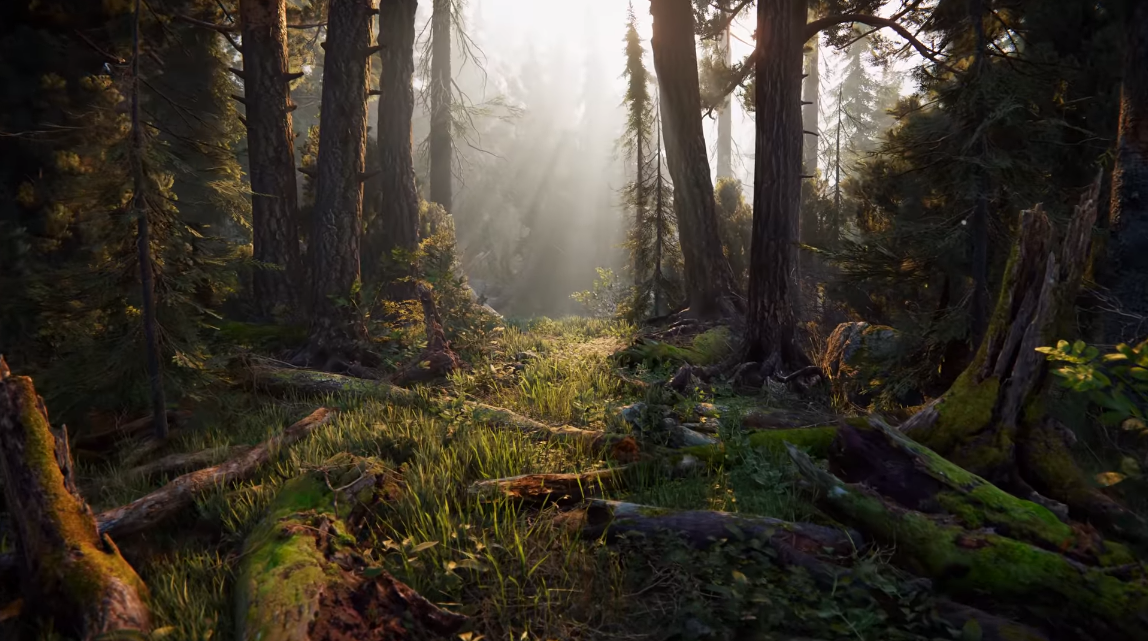
\includegraphics[width=14cm]{img/ch05/UnityGraphicsDemo.png}
\captionof{figure}[Unity Engine demo]{Unity Technology's "Book of the Dead" promotional video \cite{UnityDemoRealtimeTeaser}}
\label{fig:unity-demo-graphics}
\end{center}

New rendering-technologies that improve the quality of rendered images and performance of the rendering-process are being developed and published by both proprietary and open-source developers. A current example of a new technology recently published is NVIDIA's proprietary "RTX"-technology \cite{NVIDIARTX} that features "Hybrid Rasterization and Ray Tracing" \cite{NVIDIARayTracing} to combine raytracing and conventional rasterization in the rendering-process. A public demonstration of this new technique was shown running on the "Unreal Engine" in a short video (figure \ref{fig:unreal-demo-graphics})\cite{UnrealDemoReflections}.
\begin{center}
\noindent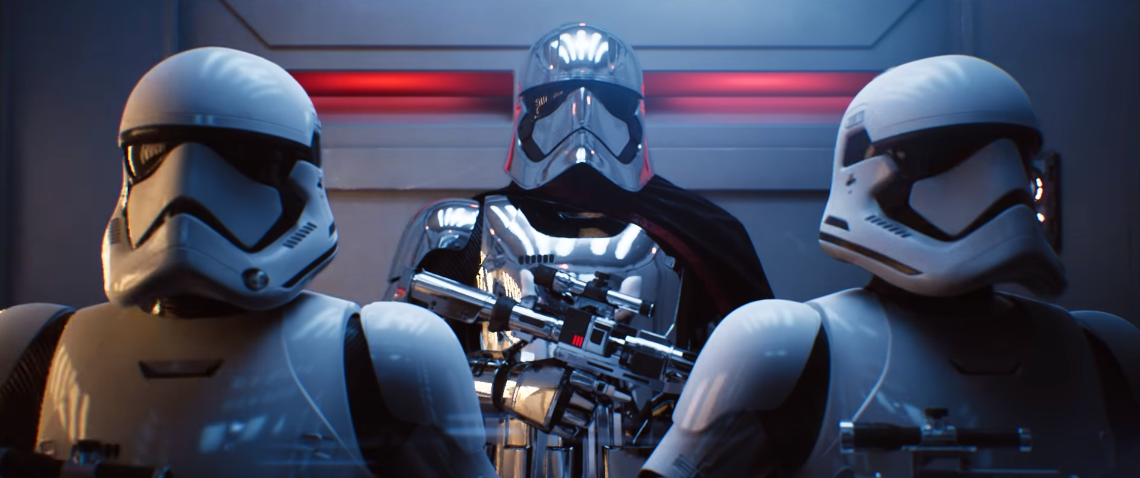
\includegraphics[width=14cm]{img/ch05/UnrealGraphicsDemo.png}
\captionof{figure}[NVIDIA RTX demo]{Demonstration of NVIDIA RTX and Microsoft DXR running on the Unreal Engine \cite{UnrealDemoReflections}}
\label{fig:unreal-demo-graphics}
\end{center}

%////////////////////////////////////////////////
\subsubsection{Choosing a Game Engine}
The decision which game engine to use to implement the concept was based on a set of factors (inspired by criteria defined by Cowan \textit{et al.} \cite{6901570}) that needed to be considered:
\begin{description}
\item [Stability] While the goal of using game engines as real-time renderers is to generate records quickly, recording sessions may take several hours. The software needs to maintain stable operation because recording sessions may run un-supervised and crashes may be detected only hours later.
\item [Crossplatform] Support of multiple platforms serves multiple purposes. First it aims to avoid platform-specific problems that may either be already existent or yet to come. Operating system updates can cause software to malfunction as was recently seen with multiple updates of the Windows operating system \cite{heiseWindowsUpdate}. Secondly, supporting multiple platforms greatly extends the potential groups of users. Users that own licenses for proprietary operating systems will be able to run the software on their current systems while users that lack licenses to proprietary operating systems may chose a free operating system. The third and very important aspect of crossplatform-capabilities is that developers only need to implement code specific to a game but no code specific to platforms. This allows to compile a game for multiple platforms without spending any time on the target platforms' specifics.
\item [Features] As this thesis' concept aims to generate labelled images of excellent quality, the game engine used for rendering said images must feature rendering capabilities that produce realistic output. This requires extensive support of post-processing features like ambient occlusion, anti-aliasing, depth-of-field and other shading-techniques.
\item [Maintenance] Software is expected to be operable for a certain period. While games may run on modern systems for few years, programs used in sophisticated fields of use like research aim to be used and developed further for many years. Programming those comes at considerable development cost which is why one important factor is the expected time a game engine enables software to run on modern systems. One way to evaluate this factor is to study when a game engine was first publicly announced, what games are being published that use the engine and in what intervals it is updated. Dependencies introduced by game engines further add to potential problems with software becoming outdated and unable to use on modern systems. 
\item [Licensing] Like most other software, game engines are usually distributed with licenses that specify under what conditions and for which purposes they may be used. Many engines that power popular games today are exclusive to their developer studios or publishers and are not available for public use (e.g. \emph{EA DICE}'s exclusive \emph{Frostbite} that powers the \emph{Battlefield} game-series or \emph{id Software LLC}'s exclusive \emph{id Tech 6} which \emph{Doom (2016)} was based on). Contrary to those, some modern proprietary game engines may be used for free for educational or private use (such as the CryEngine, Unity Engine and Unreal Engine).
\item [Community] When it comes to become acquainted with working with game engine, an active community of developers can prove very useful as documentation may become obsolete when update-cycles of game engines are very short. Open-source projects allow developers to use and learn from others' code so one may be more likely to find open-source projects for popular game engines than less popular ones.
\item [Assets] Some developers of game engines (such as Unity and Unreal Engine) offer access to free or paid assets (such as 3D models, sound and even code) that can be used in projects. Using existing assets saves time during development.
\item [Tools] Popular game engines are usually distributed with alongside with tools that streamline the development of games. Some come with feature-rich all-in-one software suites (e.g. Unity, CryEngine and Unreal Engine) that cover tasks like world-building, scripting and compiling. Others provide separate tools like world-editors, conversion-tools (to convert files to proprietary formats) or compilers (e.g. Source Engine).
\end{description}

After evaluating modern and popular game engines considering the abovementioned criteria (as shown in \ref{table:game-engines}), the Unity game engine was used for implementation of the concept of this thesis. It was chosen because of its crossplatform-capabilities \cite{UnityPlatformSupport}, regular updates (between two and four updates a month in 2018 \cite{UnityDownloadArchive}), free use for educational purposes \cite{UnityForEducation}, active community of developers \cite{UnityForum} and built-in editor-application. It features a free post-processing stack \cite{UnityPostProcessingStack} and built-in editor (shown in figure \ref{fig:unity-editor}) that allows developers to build scenes, configure objects in scenes and test their games.
\begin{center}
\noindent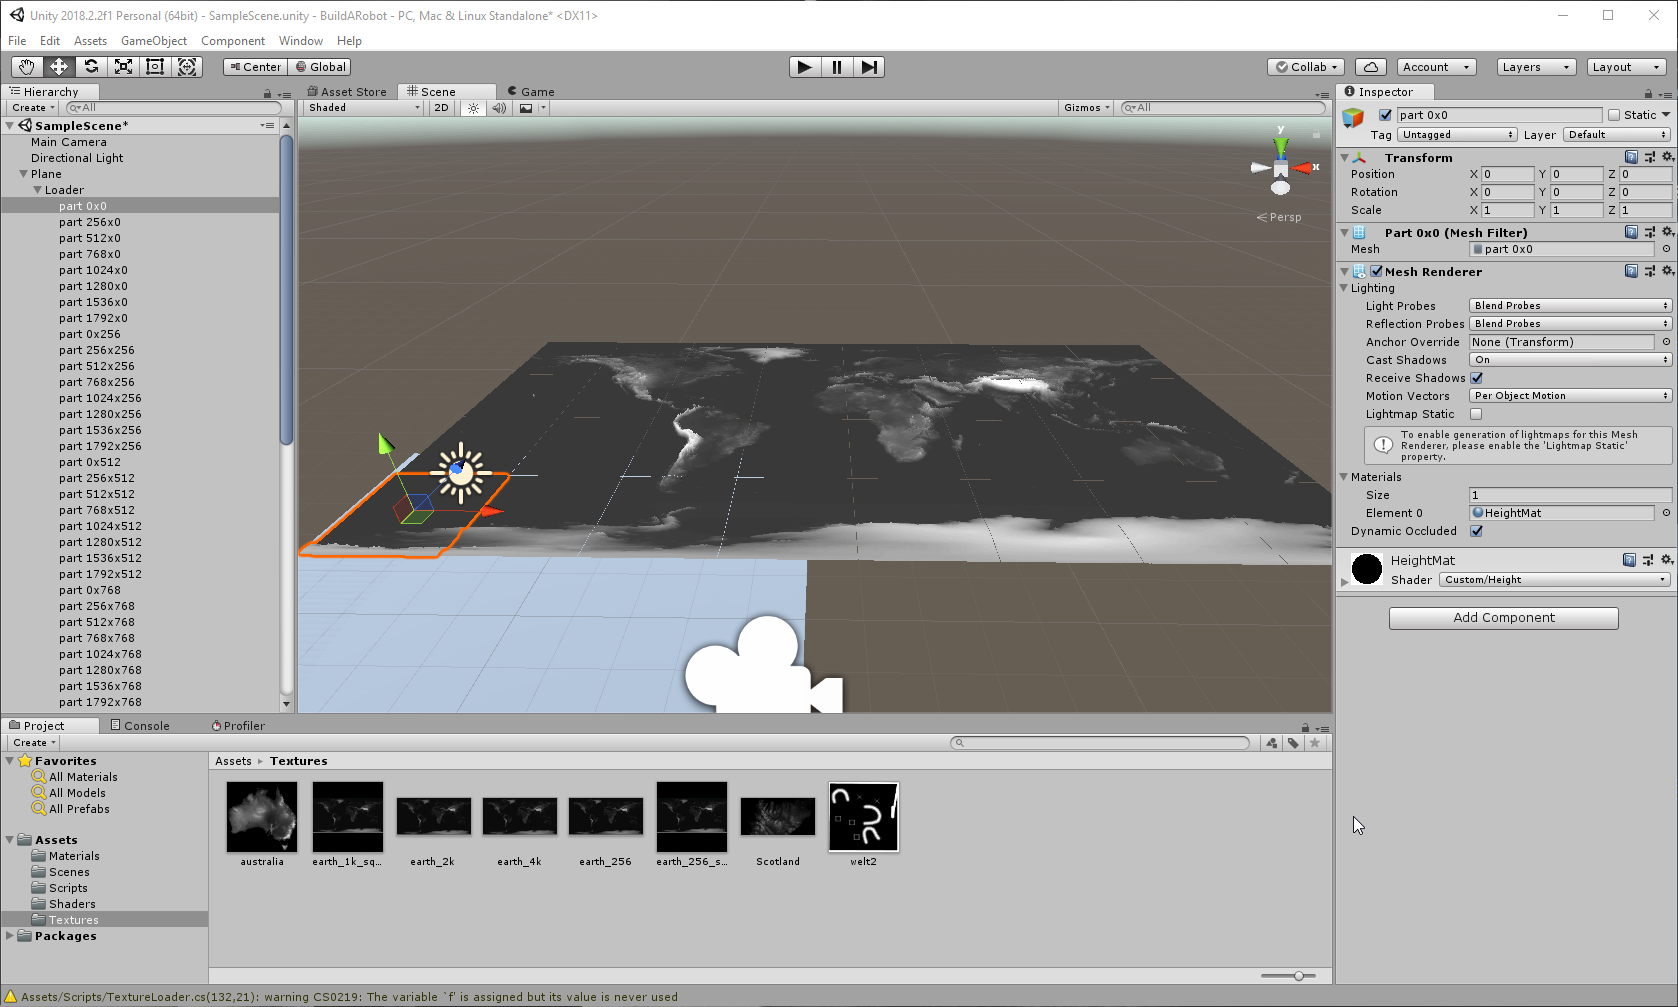
\includegraphics[width=14cm]{img/ch05/UnityScreenshot.png}
\captionof{figure}{The Unity Editor}
\label{fig:unity-editor}
\end{center}

%////////////////////////////////////////////////
\section{Designer: Building the Scene}
\subsection{Rebuilding a Real Environment}
As stated in \ref{section:goals-and-constraints} the environment used to base the scene on was the second floor of building "A" of University of Applied Sciences Mannheim. However at this time no 3D model of the floor, let alone the building existed so it had to be handcrafted using the resources that were available: a floor plan (shown in Figure \ref{fig:floor-plan-image}) and measurements taken by hand.

\begin{figure}[htp]
    % preliminary
    \sbox\twosubbox{%
      \resizebox{\dimexpr.9\textwidth-1em}{!}{%
        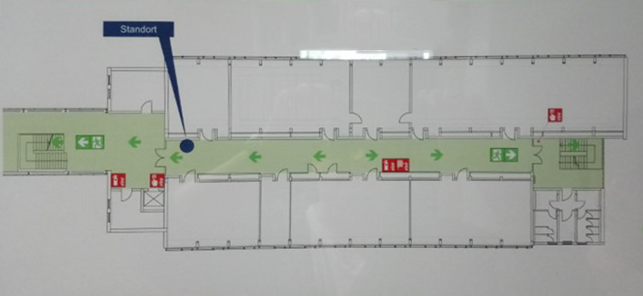
\includegraphics[height=3cm]{img/ch05/FloorPlan03_small.JPG}%
        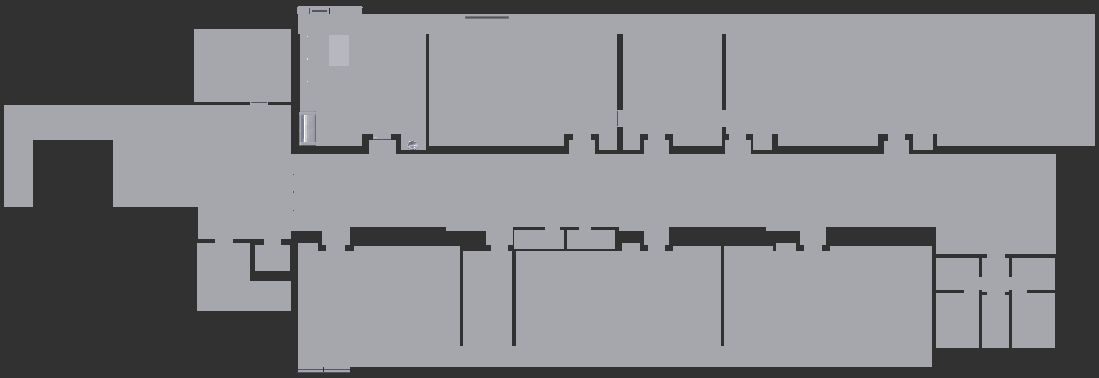
\includegraphics[height=3cm]{img/ch05/BlenderFloor01.png}%
      }%
    }
    \setlength{\twosubht}{\ht\twosubbox}
    % typeset
    \centering
    \subcaptionbox{\label{fig:floor-plan-image}}{%
      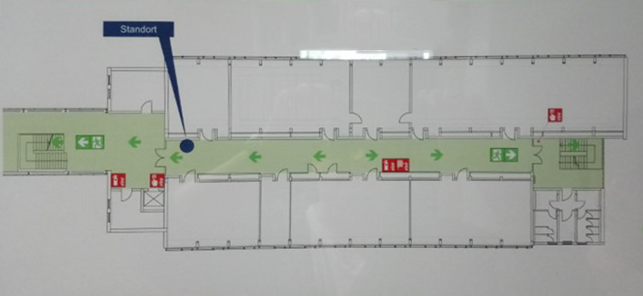
\includegraphics[height=\twosubht]{img/ch05/FloorPlan03_small.JPG}%
    }\quad
    \subcaptionbox{\label{fig:floor-plan-blender}}{%
      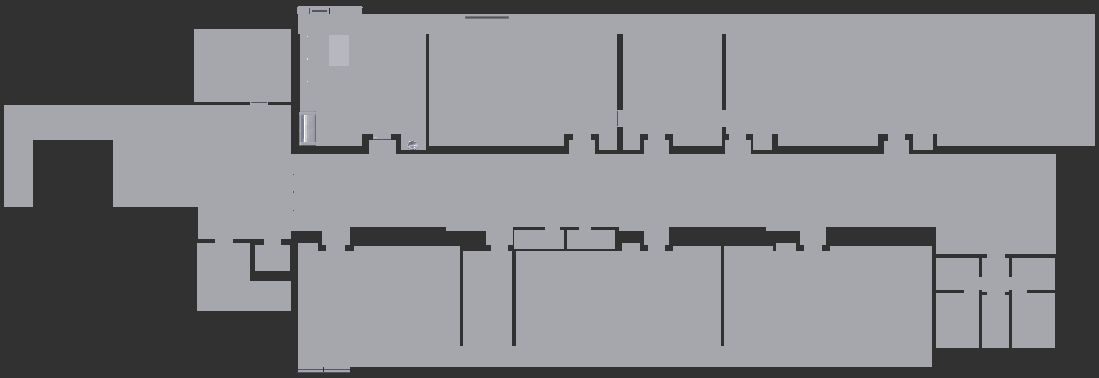
\includegraphics[height=\twosubht]{img/ch05/BlenderFloor01.png}%
    }
    \caption[Floor plan]{Floor plan, photo (\ref{fig:floor-plan-image}) and reconstruction in Blender (\ref{fig:floor-plan-blender})}
\end{figure}

\begin{figure}[htp]
    \sbox\twosubbox{%
      \resizebox{12cm}{!}{%
        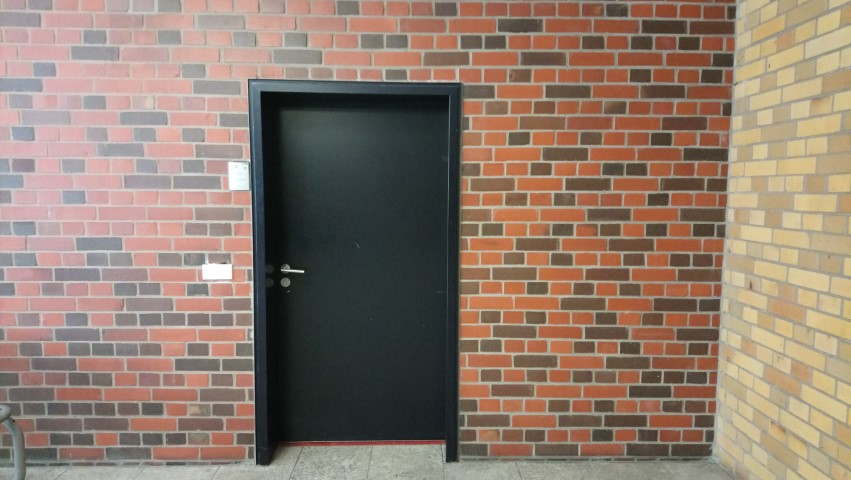
\includegraphics[height=3cm]{img/ch05/Door01_small.JPG}%
        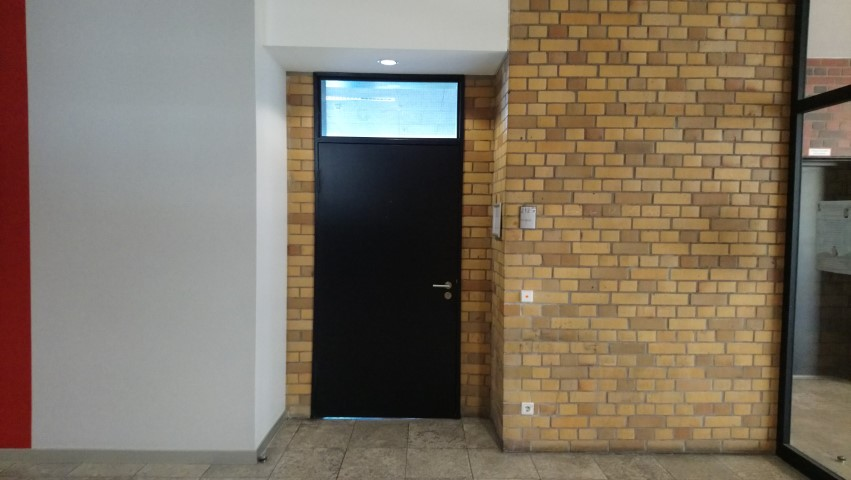
\includegraphics[height=3cm]{img/ch05/Door02_small.JPG}%
      }%
    }
    \setlength{\twosubht}{\ht\twosubbox}
    \centering
    \subcaptionbox{\label{fig:door01}}{%
      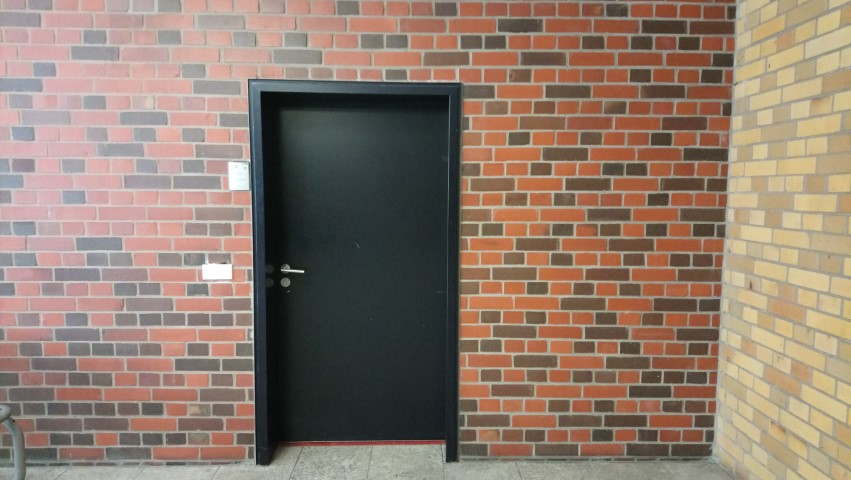
\includegraphics[height=\twosubht]{img/ch05/Door01_small.JPG}%
    }\quad
    \subcaptionbox{\label{fig:door02}}{%
      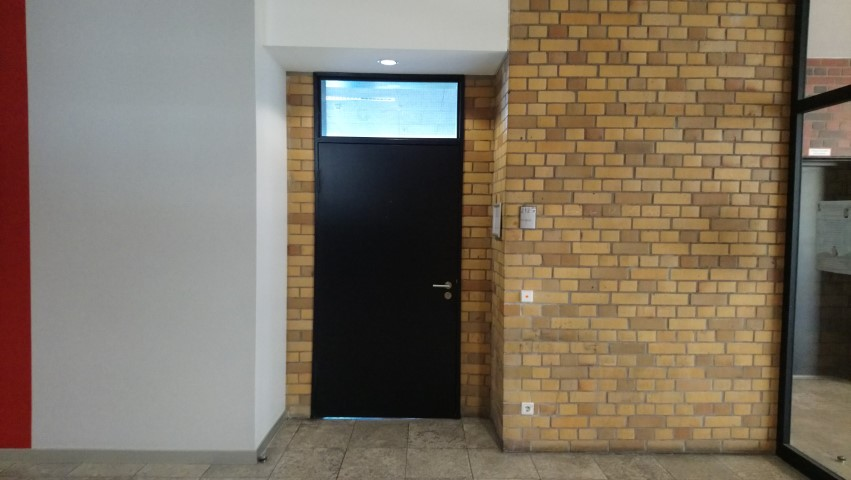
\includegraphics[height=\twosubht]{img/ch05/Door02_small.JPG}%
    }\\%quad
    \subcaptionbox{\label{fig:door03}}{%
      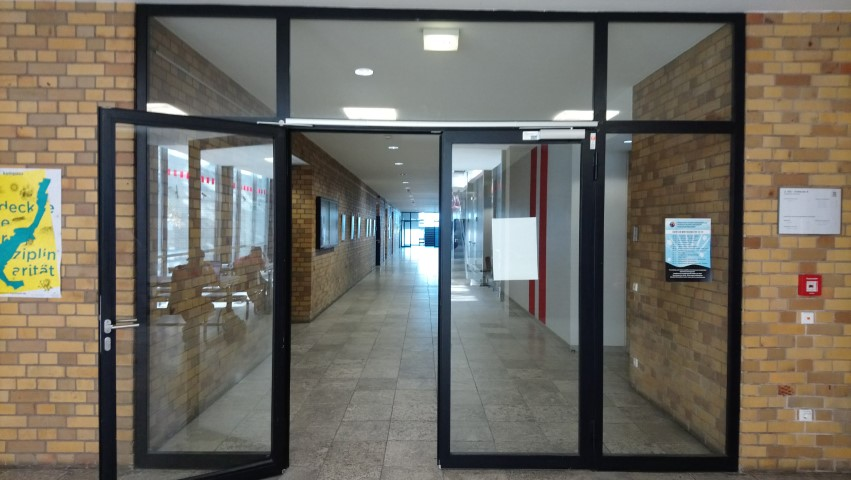
\includegraphics[height=\twosubht]{img/ch05/Door04_small.JPG}%
    }\quad
    \subcaptionbox{\label{fig:door04}}{%
      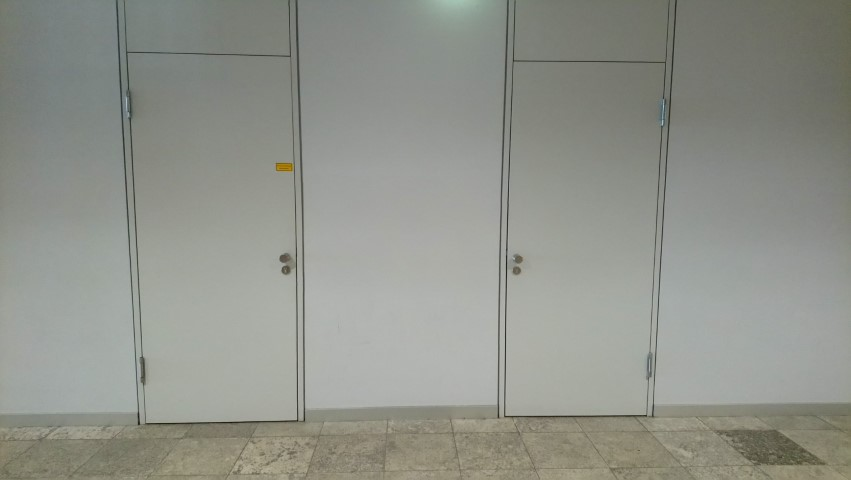
\includegraphics[height=\twosubht]{img/ch05/Door05_small.JPG}%
    }
    \caption{Various different doors on the floor}
    \label{fig:doors}
\end{figure}

Figure \ref{fig:floor-plan-blender} shows the reconstruction of the basic layout of the floor in the 3D modeling software Blender. As the goal of this implementation was to generate records used for detecting doors, special attention had to be paid to modeling the doors in this floor. This required taking measures of the doors themselves, their handles and frames as well as reconstruction of the properties of their surfaces. Figure \ref{fig:doors} shows the various doors present on this floor: office doors (shown in \ref{fig:door01}) featured metallic handles, a black and matte metal surface and were broader than most other doors. Doors to lecture rooms (\ref{fig:door02}) had blue matte metal surfaces and were not on the same level as the walls but inset into the walls. They also had glass-panels located right above them. The portals (\ref{fig:door03}) to the hallway that lead to the lecture rooms, one present at each end of the hallway, had glass doors and panels and matte black metal beams and frames. Lastly there were doors to storage rooms (\ref{fig:door04}) that did not feature great geometrical detail as the other doors did. They blended into the wall and featured knobs and hinges that were noticeably shiny.\\
The reconstructed doors could now be used to render very detailed door meshes with realistic surfaces. However other objects also had to be reconstructed: as lighting would have great influence on generated images, large window facades that cover the building's exterior and feature blinds were added to the scene. A set of other common objects present in the floor like lamps and air-conditioning pipes on the ceiling, radiators and tables were also reconstructed. For the reconstruction of the ceiling and floor tiles photos were taken of the actual tiles. They were further prepared for use in Blender and Unity by removing perspective distortion and scaling the resulting textures so they would allow infinite tiling. Normal maps automatically generated from the gray scale color of these textures added visual detail to these surfaces.\\
Figure \ref{fig:unity-scene-a205} shows the final reconstruction of room \emph{"A205"} which is the first room on the second floor of the building. It features windows with blinds that cast shadows on the walls and objects and it features obstacles (such as tables) that may occlude other objects of interest such as the blue door. The reconstructed room does not feature any chairs, even though there were chairs present in the real room. They were left out to enable robots to navigate through the room easily without having to take care of maneuvering in tight spaces between chairs. However chairs would have contributed to making the room appear more realistic as chairs may have occluded objects of interest and added to the complexity and variety of the scene overall.

\begin{center}%[t]
    %\centering
    \noindent
    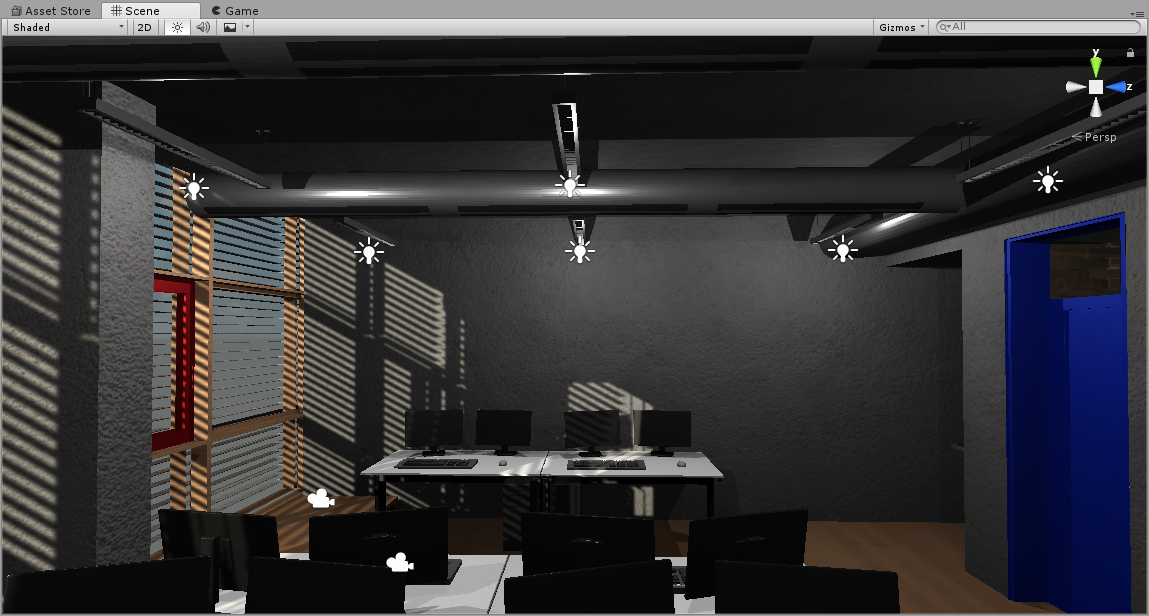
\includegraphics[width=12cm]{img/ch05/UnitySceneA205_02.png}
    \captionof{figure}{Reconstruction of room A205 in Unity Editor}
    \label{fig:unity-scene-a205}
\end{center}

%////////////////////////////////////////////////
\subsection{Adding Robots to the Scene}
Once the scene is set up, a robot is needed for \acs{AI} engineers to navigate around the scene and capture records. For this implementation the robot model "Pioneer 3AT" was chosen as the Institute of Robotics of University of Applied Sciences Mannheim works with "Pioneer"-robots and there were \ac{URDF} files of it available \cite{AmrRosConfig} online.
\subsubsection{Importing Robots}
There were few libraries that provide methods to import robots using URDF-files into Unity, an extensive one was \emph{"ROS\#"} which was developed by Siemens AG. Siemens described it to be \textit{"a set of open source software libraries and tools in C\# for communicating with ROS from .NET applications, in particular Unity3D"} \cite{RosSharp}. This project implemented connecting to ROS instances, ROS' publish/subscribe pattern and importing robots into Unity scenes, however its software design introduced some potential problems: 
\begin{enumerate}
    \item Importing robots using URDF-files was done by downloading URDF-files from running ROS-instances. The need for a running ROS-instance would add to \ac{VERE}'s system requirements.
    %ros-sharp/Unity3D/Assets/RosSharp/Scripts/Urdf/Editor/UrdfComponents/UrdfRobotExtensions.cs
    \item ROS\#'s URDF importing component required the URDF files to be present in the "Asset" folder of Unity projects. This meant that URDF files downloaded from remote locations needed to be written to disk and compressed archives that contained additional files like meshes and textures needed to be extracted to disk first.
    \item Even though robots imported by ROS\# had correct hierarchy of body parts and correct physical properties (as defined in the robots' URDF), Unity's physics engine often times failed to simulate physics at run-time, leading to robots being unable to move, falling through floors or being propelled into the air.
\end{enumerate}
To solve these problems, a library for parsing URDF-files, \emph{"URDFParser.NET"}, was implemented. The first two problems were solved by implementing a set of interfaces that represent filesystems, directories and files (shown in Figure \ref{fig:filesystem}) for local filesystems and ZIP-archives (using the open-source library \emph{"DotNetZip"} \cite{DotNetZip}) as URDF-files including meshes and textures were usually distributed as ZIP-archives. These interfaces could also be implemented to read files from remote locations such as FTP-servers or websites for future scenarios and use-cases.
\begin{center}
    \noindent
    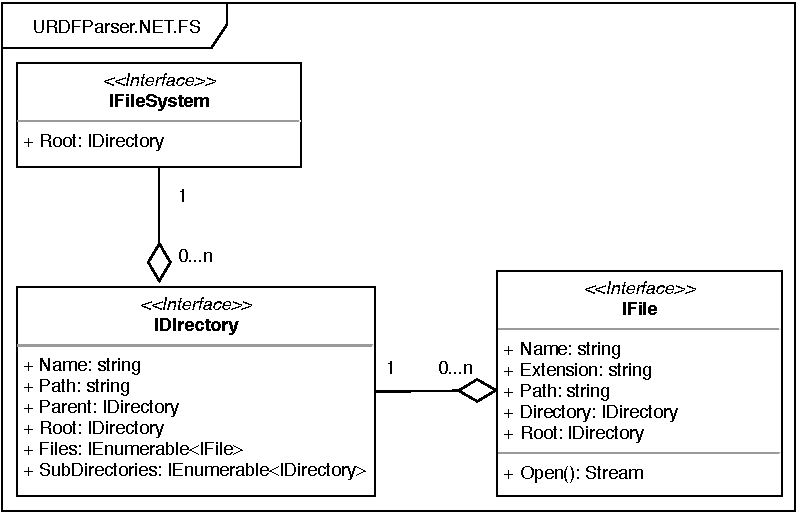
\includegraphics[width=14cm]{img/ch05/URDFParser_FileSystemInterfaces.pdf}
    \captionof{figure}{Interfaces for filesystems, directories and files}
    \label{fig:filesystem}
\end{center}
Contrary to ROS\#'s approach of interpreting hard-coded XML-elements, in URDFParser.NET parsing the URDF-files was implemented by defining \acp{DTO} for the different URDF-elements. URDF-Files could then be deserialized using these \acsp{DTO} with the \emph{"XmlSerializer"}-class provided by the .NET-Framework \cite{XmlSerializer}.\\
The third problem with ROS\#'s implementation, faulty behaviour of physical bodies (also called \emph{"rigid bodies"} in the Unity Engine), required manual adjustments to the imported robot models: rearranging the robots' hierarchy so at all times a physical object may have only one physical child object solved robots' inability to move. Ensuring that colliders of physical parts (such as wheels and chassis) did not intersect with each other eliminated the problem of robots spontaneously launching into the air. 

\subsubsection{Controlling Robots}
Robots imported into Unity needed to be controllable by \ac{AI} engineers. This could be done in different ways. some of those depending on the type of drive a specific robot featured:
\begin{description}
    \item [Wheel Drives] Robots may feature wheel-joints that can rotate on their local $x$ and $y$ axis. Rotating a wheel's $y$ axis allows to use it for steering while applying torque to its $x$ axis would move it and its connected bodies across surfaces, just like real-world wheels work. This technique can be used for most wheeled robots by limiting rotation of the $y$ axis to wheels that should not steer (e.g. the rear wheels of motor cycles).
    \item [Connected Limbs] Limbs of robots can be connected using hinge joints that allow rotating connected bodies along one or more axis. Most industrialized robots feature three or more controllable axis and could be implemented in Unity by connecting two limbs via one hinge-joint each, allowing movement in one axis. Industrialized robots operate from a fixed position in 3D space.
    \item [Legged Movement] Extending on the techniques used for implementing industrialized robots, one can combine multiple limbs to a body and move these limbs via hinge joints to simulate legged robots. The major difference from industrialized robots is that legged robots do not reside in a fixed position but move their bodies in 3D space.
\end{description}
While simulating wheel drives, connected limbs and legged movement is possible in Unity Engine and other engines, they come at the cost of complex configuration and intensive testing. An alternative to physical simulation is by simply fabricating the illusion of such, presuming that the scenario at hand does not require exact simulation of movement but allows for fabricated approximations:
\begin{itemize}
    \item Wheel drives can be reconstructed by wheel joints that allow for rotation in the $x$ and $y$ axis, however they do not require force directly applied to them for rotation . Applying directed force at a robot's body for acceleration and deceleration and applying torque force for turning would indirectly affect the wheels and thus fabricate the illusion of real wheel drives. 
    \item Connected limbs can be imitated by creating a parent-child hierarchy for each connected limb. Making use of Unity's transforms, child limbs of parent limbs will directly be affected by any change to the parent's transform: for instance, rotating the base limb of a robot arm would also effectively move all of its child limbs with it.
    \item Legged movement would be the hardest to fabricate in a way that behaves realistic. Most game engines feature animation systems that allows for replaying, looping and blending animations of complex body parts, resulting in movement that looks realistic. However it would not necessarily behave realistically as individual legs colliding with obstacles could lead to the whole body being moved, ignoring the friction of the other legs of a robot that may have contact to a surface and thus restrict movement of the robot's body.
\end{itemize}

Figure \ref{fig:pioneer3at} shows a "Pioneer 3AT" robot imported into Unity. The green cylinders represent the colliders of its wheels and it lacks any other colliders. Its only rigid body that had any mass and was simulated for gravity was its chassis. This combination of a single rigid body and one cylindrical collider for each wheel enabled the robot to appear and behave close to a real robot in the scene as neither collision with its chassis nor mass of its wheels were necessary for maneuvering it in the scene. Its wheels would turn when force is applied to its rigid body.
%\begin{center}
\begin{figure}[t]
    \centering
    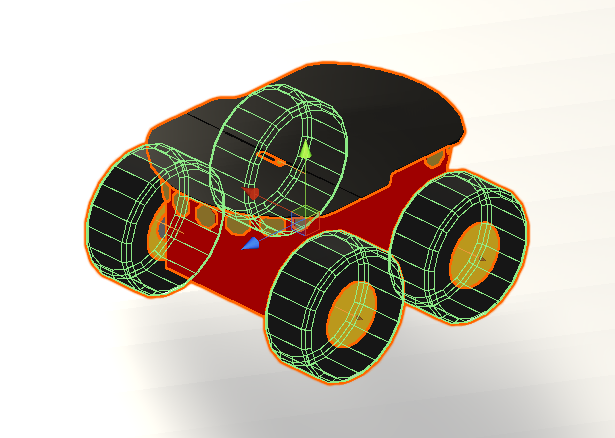
\includegraphics[width=0.39\textwidth]{img/ch05/Pioneer3AT.png}
    \captionof{figure}{A "Pioneer 3AT" robot imported into Unity}
    \label{fig:pioneer3at}
\end{figure}
%\end{center}
Unity unifies input of various different input devices by providing an extendable set of values that either buttons and axis of one or multiple input devices can be mapped to. In its default configuration, Unity maps input for movement from both digital inputs like keyboards and analog inputs like joysticks to two axis, one for horizontal and one for vertical movement. As a result, pressing the "A" or "Arrow Up" buttons on a keyboard and pushing a joystick into the positive direction of its $y$ axis would affect the vertical input axis. In scripts, this could then be accessed by a simple call to $Input.GetAxis("Vertical")$ which would return a value in the interval $[-1, 1]$ where positive values indicated a movement forwards and negative values indicated a movement backwards. Analogue to this, negative values of the horizontal axis would indicate movement to the left and positive values would indicate movement to the right.\\
In \ac{VERE}, the vertical axis for forwards and backwards movement was used to apply either a positive or negative force to the robot's body in its forward direction which would make it accelerate and decelerate. The horizontal axis was used to apply a torque force to its body, allowing it to steer. Due to the mass of the robot the applied torque force was not sufficient to move it while it was standing still, however it was strong enough to apply slight steering to the robot while it was driving, which in turn appeared realistic.

%////////////////////////////////////////////////
\section{Implementing Mutators}
The concept of this thesis proposed generating sets of diverse images by utilizing mutators to alter the appearance of single entities or whole scenes. Mutators would operate on a step-by-step basis, altering the state of an entity by each step. In this implementation, mutators would implement a simple interface \emph{IMutator} that provided methods to advance and reset itself. Three implementations of this interface were used to simplify the use of this interface for various applications: 
\begin{description}
\item [RangeMutator] Most attributes that were to be altered had numerical values that had to be incremented or decremented each step. \emph{RangeMutators} would have a \textit{FloatRange} associated to them that defined a value-range and step-size. These mutators could perform mutations on a single attribute of a single object using a value within the specified range of values and incremented or decremented this value using the specified step-size. RangeMutators would be used to manipulate most numeric values like light-intensity, the angles that doors were opened by and the orientation of the sun. The number of steps $s$ needed to complete one cycle of this mutator is $|\frac{maximum-minimum}{stepSize}|$ where $maximum$, $minimum$ and $stepSize$ are specified by a RangeMutator's FloatRange.
\item [MultiMutator] A single entity could hold many mutators and in order to group them and make them easily accessible to the MutationManager, those mutators would be added to and effectively encapsulated by \emph{MultiMutators}. Those would advance mutators in a serial fashion: it advanced the first child-mutator until the cycle of this child-mutator was completed. Then it would advance the second child-mutator by one step, reset the first one and continue advancing the first child-mutator again. The number of steps a MultiMutator needed to complete a cycle was directly dependent on the mutators it grouped. Given the set of its mutators $m$ a MultiMutator needed $\prod_{i=1}^{|m|} S(m_i)$ steps to complete a cycle, where $S(x)$ returns the number of steps a mutator $x$ needed to complete a cycle.
\item [ParallelMutator] There were cases where single mutators did not have great influence on scenes or did not have to have a whole mutation-step in a scene dedicated to them. For instance in this implementation, lamps in room A205 were mutated in parallel by using a ParallelMutator. These mutators would group other mutators like MultiMutators did, however upon mutation it would advance all of its mutators at the same time. Mutators that finished their current cycle were skipped. The number steps a ParallelMutator needed to complete a cycle was the number of steps the slowest of its mutators took to complete a cycle. ParallelMutators may have mutators of varying cycle lengths resulting in steps that few or only one of its mutators were advanced at.
\end{description}
Figure \ref{fig:classdiagram-mutators} shows the abovementioned mutators and a set of mutators that were implemented specifically to alter doors. Doors had a \emph{DoorMutator} associated to them which was a MultiMutator that encapsulated five other mutators. Four of them, \emph{DoorMaterialColorMutator}, \emph{DoorMetallicMutator}, \emph{DoorNormalMutator} and \emph{Door-SmoothnessMutator}, altered the color, "metallic" property, intensity of normal maps and "smoothness" property of a door's surface, respectively. \emph{DoorAngleMutator} changed the angle at which a door was opened.\\
Figure \ref{fig:mutated-door} illustrates how doors had been affected by the mutators. The most-right images demonstrate a case of a poorly configured mutator: the "metallic" property that controls how light is reflected on surfaces, was altered to a value that results in unrealistic appearance. Similar mutators were implemented for ceiling lights (altering the intensity and range of lights), ambient light (mutating intensity and color) and the sun (altering color, intensity and orientation).
\begin{center}
    \noindent
    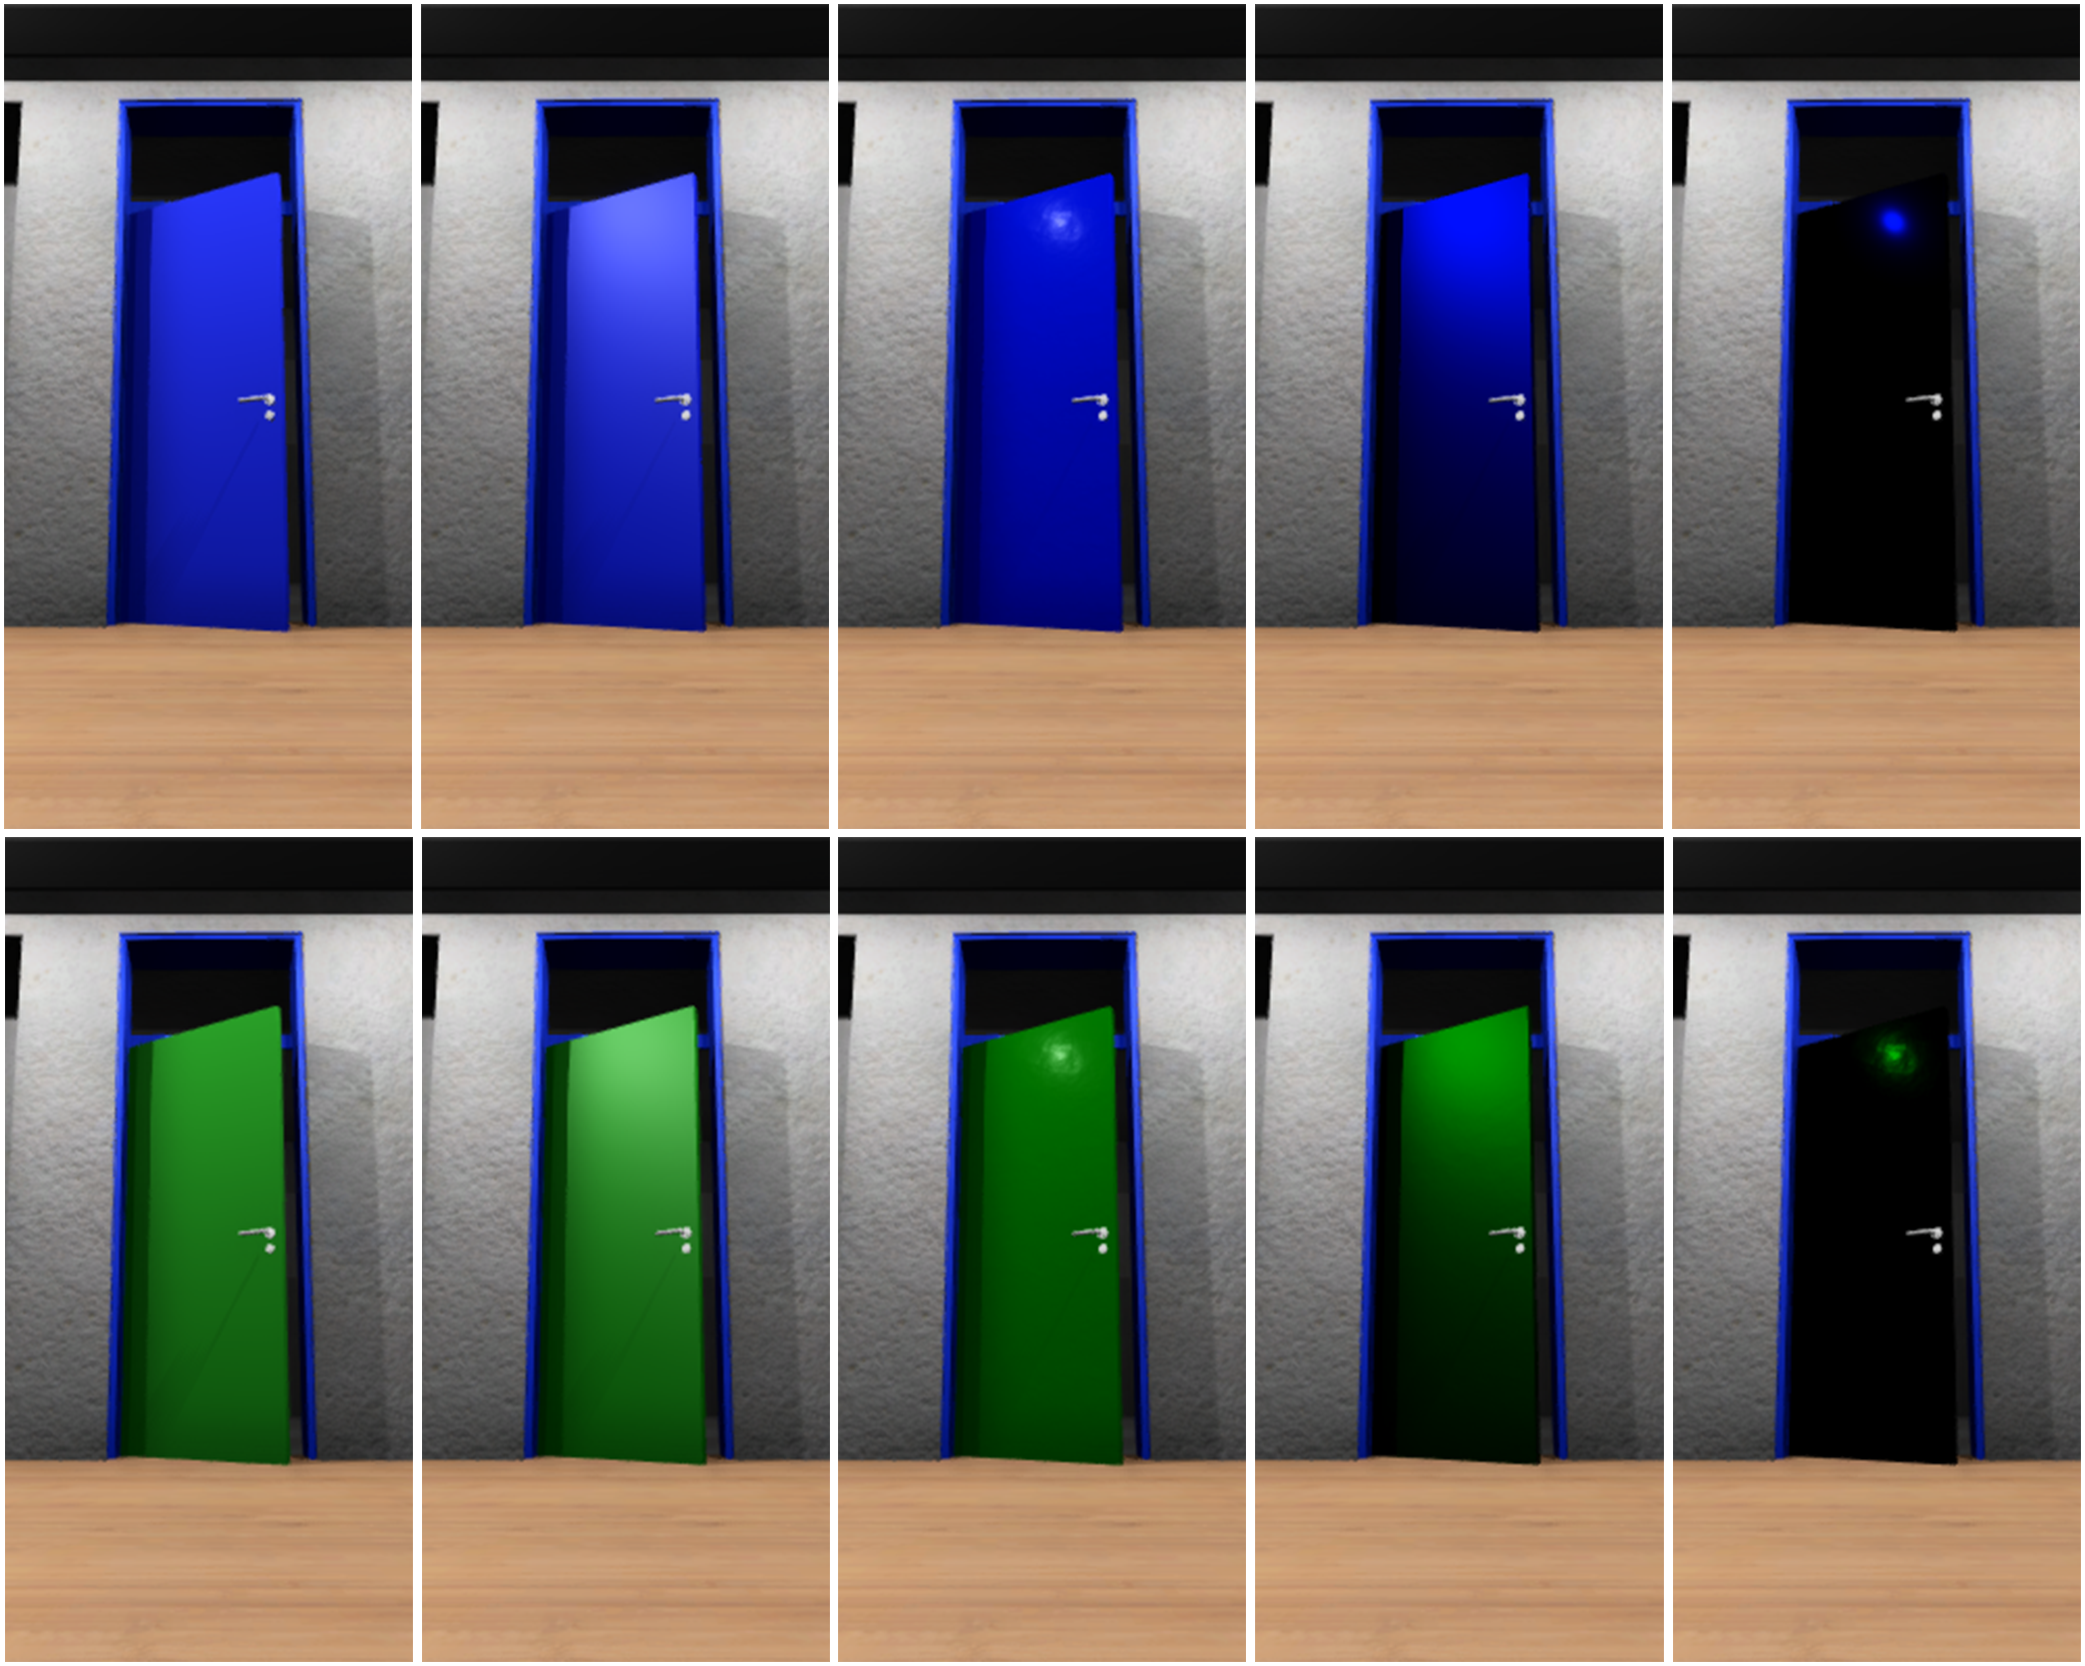
\includegraphics[width=10cm]{img/ch05/Results_Door.png}
    \captionof{figure}[Mutators applied to a door]{A door that shows mutated opening angle, color, light-reflection, normal-map and smoothness}
    \label{fig:mutated-door}
\end{center}

%////////////////////////////////////////////////
\section{Identifying Classifiers}
Proper identification of objects in captured images proved to be a non-trivial problem and the solution to this problem used in \ac{VERE} took multiple approaches until a satisfying solution was found.\\
In order to specify which objects were of interest and shall be identified in captured images, a "Taggable"-component, that had a "Label Name"-attribute that would be treated as a classifier, was implemented and added each relevant object in a scene. The next sections will present the working principles of selected approaches that were implemented and tested and their qualities and drawbacks.

\subsection{Approach I: Using Projection and Raycasting}
The first approach to identifying which objects were visible from a given camera's perspective was to try to cast rays to each "tagged" object and, if hit, project its position from world space into the screen space of the camera. If an object was not hit, it would be occluded by other objects, if the projection from world- to screen space could not be made, the object would not be in the camera's field-of-view and thus not be visible. Cameras in the Unity Engine provide the \emph{"WorldToScreenPoint"} \cite{UnityDocsCamera} method that performs the projection from world space to screen space.\\
Objects in the Unity Engine have transforms that specify location, rotation and scale. These do not translate to colliders of objects though and can not directly be used to determine if an object is hit by a raycast or not as an object may have no colliders that cover its origin: for instance a tire may have its origin at its center so a ray-cast to its origin would not necessarily hit any of its colliders. Therefore, the projection approach needed to consider objects' colliders. A solution to this was to define a set of points to test for along the edges and on the surfaces of colliders: an algorithm would create a point for each vertex of a collider and add a configurable amount of points along edges and surfaces. Each point of these sets could then be tested for using raycasting and projection.\\
Figure \ref{fig:w2s-labelling} shows a door that had these points added to its collider (for a single face) as boxes that were grey and would turn red if proven to be visible by raycasting and projection. Additionally, a red rectangle indicated a region that spanned across all detected points. As can be seen in \ref{fig:labelling01}, \ref{fig:labelling02} and \ref{fig:labelling05} this approach worked reliably in cases where the door took up enough screen space to show multiple points horizontally. In cases where only few points were visible horizontally, as seen in \ref{fig:labelling04}, the indicated region became very thin and in some cases was only one pixel wide, even though parts of the geometry that were not covered by the indicated region were in fact visible. Figures \ref{fig:labelling05}, \ref{fig:labelling06} and \ref{fig:labelling04} were captured while increasing the distance between the camera and the door. These images illustrate a quality of this approach: as long as objects are not fully occluded, parts of them may still be visible from great distance. Due to the decrease in detail in images with the increase of distance from the camera to objects, this may not be usable for training object-recognition software though: distant objects may accommodate for few, if any, pixels in an image and thus be nearly indistinguishable other objects or become hard to identify. This could be solved by limiting the range of rays.\\
A great problem with this approach proved to be its implications on performance: for each object, all of its points needed to be ray-casted for and, if not occluded, projected to the screen. The time it took to test for all objects in a scene was depending on the total amount of objects in a scene, thus the more detailed and larger a scene became, the more time was required to test which objects were visible.\\
\begin{figure}[htp]
    % preliminary
    \sbox\twosubbox{%
      \resizebox{14cm}{!}{%
        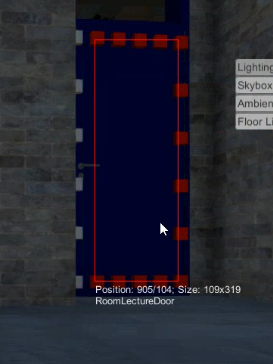
\includegraphics[height=6cm]{img/ch05/Labelling_W2S01a.png}%
        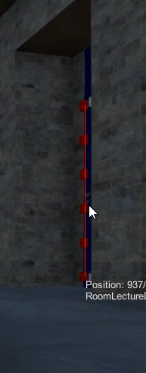
\includegraphics[height=6cm]{img/ch05/Labelling_W2S02a.png}%
        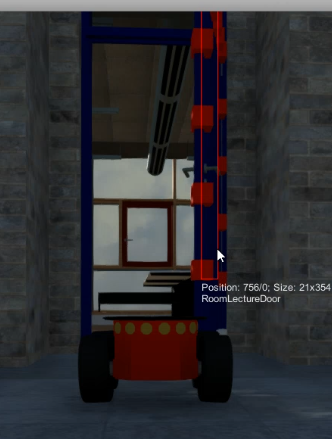
\includegraphics[height=6cm]{img/ch05/Labelling_W2S03.png}%
        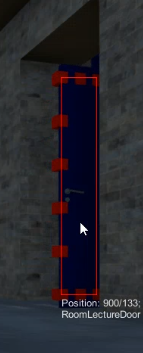
\includegraphics[height=6cm]{img/ch05/Labelling_W2S04a.png}%
        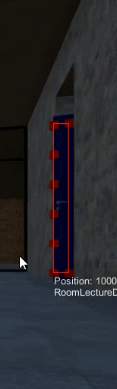
\includegraphics[height=6cm]{img/ch05/Labelling_W2S05a.png}%
        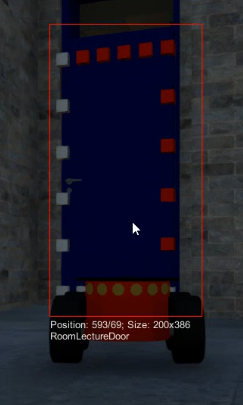
\includegraphics[height=6cm]{img/ch05/Labelling_W2S06.png}%
        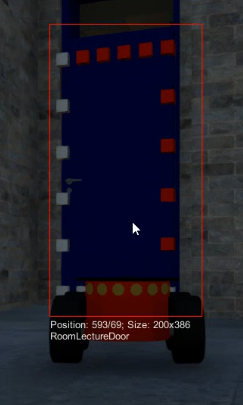
\includegraphics[height=6cm]{img/ch05/Labelling_W2S06.png}%
      }%
    }
    \setlength{\twosubht}{\ht\twosubbox}
    % typeset
    \centering
    \subcaptionbox{\label{fig:labelling01}}{%
      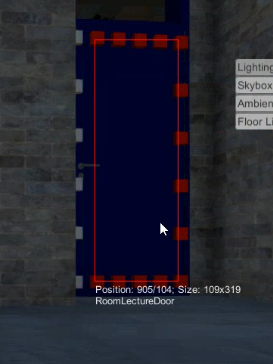
\includegraphics[height=\twosubht]{img/ch05/Labelling_W2S01a.png}%
    }\quad
    \subcaptionbox{\label{fig:labelling02}}{%
      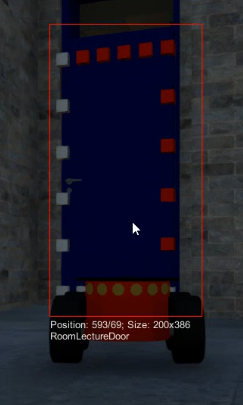
\includegraphics[height=\twosubht]{img/ch05/Labelling_W2S06.png}%
    }\quad
    \subcaptionbox{\label{fig:labelling03}}{%
      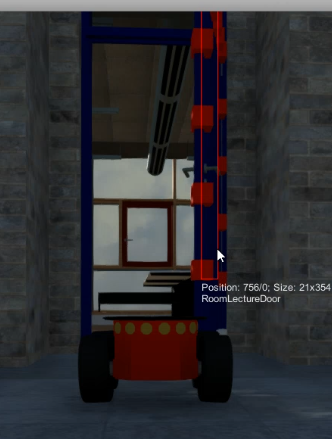
\includegraphics[height=\twosubht]{img/ch05/Labelling_W2S03.png}%
    }\quad
    \subcaptionbox{\label{fig:labelling05}}{%
      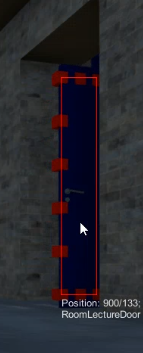
\includegraphics[height=\twosubht]{img/ch05/Labelling_W2S04a.png}%
    }\quad
    \subcaptionbox{\label{fig:labelling06}}{%
      \includegraphics[height=\twosubht]{img/ch05/Labelling_W2S05a.png}%
    }\quad
    \subcaptionbox{\label{fig:labelling04}}{%
      \includegraphics[height=\twosubht]{img/ch05/Labelling_W2S02a.png}%
    }
    \caption[Raycasting and projection approach]{Drawing regions of the identified door from multiple perspectives}
    \label{fig:w2s-labelling}
\end{figure}
Another problem was determining how to create the points on colliders to test for: complex colliders, such as mesh-colliders, could have any shape and any distance from one vertex to another. Those could also have shapes that have vertices that may be occluded by faces and thus never or just rarely be visible, such as convex shapes. As a result, testing for them potentially wasted valuable computing time. Even simple shapes such as cubes and cylinders were not trivial to test for as with increasing scale of objects, the distance between vertices may grow too large to test for: for instance a cube that had an edge length of one meter and had points added to its vertices, three points on each edge and four points evenly distributed on each face, the distance between any neighbouring points would be 25 centimeters. Scaling the cube by a factor of 100 would also scale the distance between said points by 100 and result in neighbouring points being 25 meters away from each other.\\
Solving this problem would require dynamically generating points on colliders, taking the shape and scale of an object into account.

% ** Raycasting
\subsection{Approach II: Casting Rays From Screen Space}
After using raycasting on every object in the first approach raised performance-concerns, an alternative solution needed to be found. Ideally, a second approach should take the same time to test for visible objects on screen each time it was run and not be influenced by the total amount of objects in a scene.\\
The second approach to identifying objects on images aimed to imitate how humans would process captured images: humans would actually exclusively look at the images presented to them as no other information would be available to them. They may not know about all the other objects in a scene that are not visible in an image and they would most likely not recognize distant objects in images very well due to how few pixels would accommodate for them.\\
Therefore the algorithm implemented in this approach (shown in algorithm \ref{algo:raycasting-screenspace}) scan-ned the scene from the active camera's perspective in a grid-like fashion. It would use the camera an image was taken with, the \emph{scan-resolution} that defined how many rays it would cast horizontally and vertically and the screen-resolution in pixels and then cast rays that originated from the camera's origin and went through points in screen space, going from top to bottom and left to right (shown in Figure \ref{fig:rclabelling02}). If a cast hit a collider [of a tagged object] it would check whether the same object was already hit before and retrieve a rectangle associated with the object, or create a new rectangle for the object. This rectangle would be extended so that it would contain the screen-coordinate that was used to cast the ray. Once the algorithm finished casting rays it would return a map with rectangles describing regions on screen covered by a single object each associated with their corresponding object (seen in Figure \ref{fig:rclabelling05}). By defining a threshold of the minimum size rectangles needed to be, too small rectangle were discarded, allowing to effectively skip objects that were either too far away from the camera or occluded.\\
\begin{figure}[htp]
    % preliminary
    \sbox\twosubbox{%
      \resizebox{14cm}{!}{%
        \includegraphics[height=3cm]{img/ch05/RaycastingAlgorithm01.png}%
        \includegraphics[height=3cm]{img/ch05/RaycastingAlgorithm02.png}%
        \includegraphics[height=3cm]{img/ch05/RaycastingAlgorithm03.png}%
        \includegraphics[height=3cm]{img/ch05/RaycastingAlgorithm03.png}%
        \includegraphics[height=3cm]{img/ch05/RaycastingAlgorithm03.png}%
      }%
    }
    \setlength{\twosubht}{\ht\twosubbox}
    % typeset
    \centering
    %\subcaptionbox{\label{fig:rclabelling01}}{%
    %  \includegraphics[height=\twosubht]{img/ch05/RaycastingAlgorithm01.png}%
    %}\quad
    \subcaptionbox{\label{fig:rclabelling02}}{%
      \includegraphics[height=\twosubht]{img/ch05/RaycastingAlgorithm02.png}%
    }\quad
    \subcaptionbox{\label{fig:rclabelling03}}{%
      \includegraphics[height=\twosubht]{img/ch05/RaycastingAlgorithm03.png}%
    }\quad%\\
    \subcaptionbox{\label{fig:rclabelling05}}{%
      \includegraphics[height=\twosubht]{img/ch05/RaycastingAlgorithm04.png}%
    }\quad
    \subcaptionbox{\label{fig:rclabelling06}}{%
      \includegraphics[height=\twosubht]{img/ch05/RaycastingAlgorithm05.png}%
    }
    \caption{Various stages the raycasting algorithm went through}
    %\caption{Ray-Casting algorithm: division of the original image (\ref{fig:rclabelling01}) by horizontal and vertical lines (\ref{fig:rclabelling02}), detection of objects hit by rays (\ref{fig:rclabelling03}), calculating rectangles that cover objects (\ref{fig:rclabelling05}) and extending them to include neighboured area (\ref{fig:rclabelling06})}
    \label{fig:rc-labelling}
\end{figure}


In practice, these rectangles usually would not fully cover objects which is why in the implementation of the algorithm, an option was added to extend the width and height of the rectangles by an adjustable factor, resulting in rectangles that fully covered objects and even included neighbouring area (like parts of the ceiling, wall and floor in Figure \ref{fig:rclabelling06}). Including neighbouring areas in these rectangles adds context to the found objects that may contribute to the quality of detection of object-recognition software. For doors, in this implementation this factor was set to $1.5 \times 1.3$ for width and height, respectively, to accommodate for the distinctive shape of doors.\\
The scan-resolution effectively determines the level of detail that should be detected at which distance and the position of its rays depend on the horizontal and vertical field of view of the camera that is used. The vertical and horizontal field of view of a given camera can be calculated using the focal-length $f$ and sensor-size $d$ (provided by Unity's \emph{physical camera} feature) and the general formula for calculating the angle of view \cite{WikipediaAngleOfView}:
\begin{equation}\alpha = 2 \arctan(\frac{d}{2f})\end{equation}
Unity's camera will have a \SI{36}mm $\times$ \SI{24}{mm} sensor-size and \SI{20.78}{mm} focal-length by default, resulting in a field of view of $82 \times 60$ degrees horizontally and vertically. The maximum distance between two rays being one meter from the camera can be determined by calculating the distance $m$ between any unit-vector (e.g. $v_f = (0, 0, 1)^T$) and the same vector with a rotation along the $y$ and $x$ axis by the scan-resolution $r$ applied to it:\\
\begin{equation}
    \begin{split}
        \alpha & = x_f / x_r, \beta = y_f / y_r\\
        v_r & = \begin{pmatrix}\cos(\alpha) & 0 & -\sin(\alpha) \\ 0 & 1 & 0 \\ \sin(\alpha) & 0 & \cos(\alpha)\end{pmatrix} \times
        \begin{pmatrix}1 & 0 & 0 \\ 0 & \cos(\beta) & \sin(\beta) \\ 0 & -\sin(\beta) & \cos(\beta)\end{pmatrix} \times
        \begin{pmatrix}0 \\ 0 \\ 1\end{pmatrix}\\
            & = \begin{pmatrix}(-\sin(\alpha)) \cos(\beta) \\ \sin(\beta) \\ \cos(\alpha)\end{pmatrix}\\
        m   &= || v_f - v_r || = \sqrt{\Big[\sin(\alpha) \big[-\cos(\beta)\big]\Big]^2 + \sin(\beta)^2 + \cos(\alpha)^2}
    \end{split}
\end{equation}

Using a rather rough scan-resolution of $10 \times 5$, at any distance of $n$ meters from the camera, neighbouring rays would be at most $0.866 \times n$ meters away from each other. Such rough scan-resolutions may be used to identify large objects in images and skip smaller ones.\\
The execution-time this algorithm needed to identify objects in images was not depending on the number of tagged objects in the scene anymore but instead depended on the time needed to perform a fixed set of ray-casts. This allowed scenes to grow in size and complexity as the number of tagged objects would not influence the labelling-process anymore. In order to run this algorithm in real-time, a maximum distance had to be defined so that casting individual rays was deterministic. Depending on the scenario at hand, this limit should be set to the highest distance the object-recognition should still be able to detect objects at. Also, by defining appropriate scan-resolutions, the resulting regions would not include objects that were too far away from the camera or only had small parts of them visible.

\section{Generating Datasets}
Right after loading a scene \ac{VERE} created a list of all distinct labels associated to tagged objects. When it saved captured images it created a JSON file that included information about the position and rotation of the camera that was used to capture the image and a list of identified objects along with the position and size (in pixels) of their associated region in the image and their label. It also saved a textfile for each image that can be used with the neural network framework \emph{"Darknet"}. Sample output is shown in \ref{chap:appendix-output}.\\
In order to shorten the duration of the recording process, identification of objects in the scene was only performed once per mutation cycle as the robot did not move during the capture process. However this optimization did not take mutators into account that altered the geometry or transforms of objects, potentially leading to inaccurate detection regions.

\subsubsection{Inspecting the Generated Output}
To verify the correctness of the output generated by \ac{VERE} an application was needed that parsed the generated files and visualized the regions of identified objects. A desktop application was implemented under the working title \emph{VERE-Viewer} (shown in Figure \ref{fig:vere-viewer}).
\begin{center}
\noindent\includegraphics[width=14cm]{img/ch05/VERE_Viewer_Application02.png}
\captionof{figure}[The VERE-Viewer application]{VERE-Viewer visualizing regions of identified objects}
\label{fig:vere-viewer}
\end{center}
It utilized components provided by the .NET Framework for its user interface and because both \ac{VERE} and VERE-Viewer were written in C\#, parts of \ac{VERE}'s code (such as the classes of the \acp{DTO} used for meta files) could be used in the viewer application.

%////////////////////////////////////////////////
\section{Performance of the Software}
There were several factors that had an impact on \ac{VERE}'s performance. Aside from the configurable parameters (scan resolution and screen or image resolution), the hardware \ac{VERE} would run on limited its performance. Contrary to regular games it did not only render frames to screen but captured an image each frame and saved it along with meta data. Rendering frames utilized the GPU while casting rays to identify objects was performed on the CPU. Lastly, saving the records to disk required a drive that handled writing multiple files in short intervals well.\\
To test \ac{VERE} it was run on two machines with different hardware:
\begin{itemize}
    \item Machine \#1 featured a \textit{Intel i5-2310} CPU, \textit{NVIDIA GeForce GTX 760} GPU and a \textit{Kingston A400} SSD.
    \item Machine \#2 featured a \textit{AMD Ryzen 7 1700X} CPU, \textit{NVIDIA GeForce GTX 1080} GPU and a \textit{Western Digital WDS512G1X0C} M.2 SSD.
\end{itemize}
\newcommand{\minitab}[2][l]{\begin{tabular}{#1}#2\end{tabular}}
\begin{table}[h]
    \centering
    \begin{tabular}{c|c|r|r|r|r|r}
        \toprule
              \thead{$Machine$} & \thead{$Image$\\$Resolution$} & \thead{$Cycle \#1 (s)$} & \thead{$Cycle \#2 (s)$} & \thead{$Cycle \#3 (s)$} & \thead{$Cycle$\\$Average (s)$} & \thead{$Captures$ \textbackslash $s$} \\
        \midrule
            \multirow{3}*{\#1} & $640 \times 360$ & $49.64$ & $53.97$ & $51.41$ & $51.67$ & $18.79$ \\
            & $1920 \times 1080$ & $260.32$ & $272.01$ & $287.14$ & $273.16$ & $3.55$ \\
            & $3840 \times 2160$ & $871.69$ & $903.18$ & $899.74$ & $891.54$ & $1.09$ \\
        \midrule
            \multirow{3}*{\#2} & $640 \times 360$ & $39.94$ & $41.64$ & $39.67$ & $40.42$ & $24.02$ \\
            & $1920 \times 1080$ & $149.33$ & $142.25$ & $144.77$ & $145.45$ & $6.68$ \\
            & $3840 \times 2160$ & $501.56$ & $526.10$ & $537.65$ & $521.77$ & $1.86$ \\
        \bottomrule
    \end{tabular}
    \caption[Comparison of recording sessions]{Recording sessions with different image resolutions on different machines}
    \label{table:vere-performance}
\end{table}
Table \ref{table:vere-performance} shows how \ac{VERE} performed on this hardware in automatic mode (shown in detail in section \ref{ch04-control-flow}), completing three mutation-cycles with images using a very low resolution ($640 \times 360$ pixels), a common resolution used in modern monitors ($1920 \times 1080$ pixels, commonly referred to as \textit{"Full HD"} and \textit{"1080p"}) and a very high resolution that is used in modern high end displays (also known as \textit{"4K UHD"} and \textit{"4K"}). The scan resolution chosen was $200 \times 50$.
\chapter{Summary}
\label{chap:summary}
This chapter summarizes the concept presented in Chapter \ref{chap:conceptual-design} and the implementation thereof shown in Chapter \ref{chap:implementations}.

\section{Concept}
The concept presented in \ref{chap:conceptual-design} describes a software environment that has a virtual environment and robot at its core. Two groups of users interact with this system: designers create and configure scenes and objects therein while \ac{AI} engineers execute the software to navigate virtual robots and generate sets of records that are composed of images and a set of located classes. To generate diverse sets of images, mutators are added to objects in the scene. These alter attributes of objects such as light intensity. The concept assumes that certain tasks are specific to implementations such as capturing images and identifying objects in captured images. Furthermore, it defines two modes of operations that \ac{AI} engineers can enter: a manual mode allows them to navigate robots themselves while an automatic mode can be entered to have a robot ride along paths capturing images.\\
The concept deduces components from the abovementioned activities and provides a basic software architecture that specific implementations shall comply with. It is designed to be operating system, platform and framework agnostic.

\section{Implementation}
Chapter \ref{chap:implementations} shows an exemplaric implementation of the aforementioned concept under the working title "\ac{VERE}". The chapter starts with explanation why VERE makes use of game engines to implement the concept and how a game engine can be chosen for a specific scenario by evaluating certain criteria. For this implementation the Unity Engine was used because of its feature-rich editor, free use for educational purposes and its crossplatform-capabilities.\\
The environment used in the scene was the second floor of building "A" of the University of Applied Sciences Mannheim and was reconstructed using Blender and imported into Unity along with common objects present in the floor such as ceiling lights, radiators and desks. Based on another thesis that implemented object detection of doors, the goal of this implementation is to generate images of those. Therefore special attention was paid to their reconstruction.\\
The robot that was used in the scene was the "Pioneer 3AT" wheeled robot. To import it into the Unity scene, a custom parser for \ac{URDF} files was written and used in conjunction with an existing open-source solution that assembled the individual parts of the robot from the interpreted files in the scene. The chapter presents several ways to control robots in Unity and states that a non-realistic control was used because realistic movement was not of high priority in the scenario.\\
Special classes of mutators were implemented to group mutators and allow for different ways to advance mutations: ParallelMutators advance several mutators at once while MultiMutators iterate through all combinations of mutations and ensure that each of them can be captured at least once. Building up on those, more complex mutators, like the DoorMutator that consists of five other mutators, are shown.\\
A central task that is left open for implementation by the concept is identifying objects. Two different approaches are shown that were implemented and tested: one tried to cast rays to all objects in a scene and project them to the screen and an object would be deemed visible if it passed both of these tests. A second approach was implemented that imitated the way humans process images: dividing an image into regions by horizontal and vertical intervals, it would send rays originating from the camera into the scene and any object that was hit would be deemed visible in the image.\\
VERE generates records that are composed of PNG images, meta-data in JSON files and text files for use with the \textit{"Darknet"} framework. In order to inspect those files, a helper application under the working title \emph{"VERE-Viewer"} was implemented. Lastly, \ac{VERE} was tested by running it on two machines using different image resolutions to find out how they impact its performance. 
\chapter{Conclusion}
\label{chap:conclusion}
% Abschließende Bewertung!
The goal of the thesis was to develop a concept for a software system that allows to generate diverse sets of labelled images of virtual environment using virtual robots that can be used for training \acp{CNN}. This concept defines abstract parts of a software architecture and thus is very flexible in the ways it can be implemented. Parts of it (such as the CaptureController) can even be implemented to run on multiple machines. Due to the concept being operating system, platform and framework agnostic, it can be implemented for a wide range of machines. Its high flexibility comes with one drawback though: demanding tasks that are not trivial to implement (such as identifying objects in images) need to be solved again for each implementation.\\
The implementation of this concept, \ac{VERE}, is operable in that it produces images, identifies objects in them and alters scenes stepwise, resulting in diverse datasets. In order to determine if the images are usable for training with \acp{CNN}, testing needs to be done. Also \ac{VERE}'s parameters (such as image resolution and scan resolution) need to be adjusted by testing various configurations and examining the output generated by actual \acp{CNN}: \acp{CNN} may not (yet) require high resolution images to produce satisfying results.\\
During the implementation of \ac{VERE} it became clear that this software required expert knowledge and skills from various sophisticated fields: a single person trying to become acquainted with and apply these proved to be difficult considering the time constraint. Reconstructing a detailed environment showed to require a considerable amount of effort and time: taking measure of the floor, windows, doors, door frames, desks and other objects was time-consuming but required for the implementation. The reconstruction was not limited to meshes but also included materials: photos needed to be taken of real surfaces (such as the floor and ceiling tiles), edited, imported into Unity and added to the individual objects in the scene. There are approaches that may greatly simplify these tasks:
\begin{description}
    \item [Procedurally Generated Geometry] Procedurally generating scenes by defining rules that specify how re-usable pieces of geometry and entities (\emph{prefabs}) are appended to form a scene is already used in games today \cite{strafeWiki}. Once these rules and prefabs are created, an arbitrary amount of scenes could be generated in a fraction of the time it would take designers to produce them. Future work on the concept presented in this thesis could evaluate if this approach is feasible and produces realistic results. Aspects that are of particular interest would be the complexity of the workflow of this approach and how it could be implemented so rules that were defined and prefabs that were created would be portable to multiple scenarios.
    \item [Using Pointcloud Data] To decrease the time spent on reconstructing real environments, pointcloud data of scans of existing environments could be used as blueprints. These would naturally contain relevant measures needed to reconstruct geometry, such as the dimensions of walls and floors. While this may sound trivial, gathering this data requires time and access to the environment and these may be limited resources. Reconstruction of environments by using pointcloud data is subject to current research and could be an interesting approach that future research might pick up and work on \cite{MINEO201981}. 
\end{description}
Implementing the concept should be done in a team of people that are experts at the tasks involved. Also by splitting tasks of the roles introduced by the concept (\textit{designers} and \textit{\ac{AI} engineers}) and sharing them with additional roles, work could be parallelized: \textit{3D artists} could reconstruct existing environments or model new ones while \textit{designers} specify, place and configure mutators required in a scene. \textit{Programmers} would implement and test those. \ac{AI} experts could use the time, that 3D artists, designers and programmers take to set up a scene, to develop a \ac{CNN} specific to the needs of the scenario. 
% ------------------------------------------------------------------

\label{lastpage}

% Neue Seite
\cleardoublepage

% Backmatter mit normalem Zeilenabstand setzen
\singlespacing

% Römische Ziffern für die "Back-Matter", fortlaufend mit "Front-Matter"
\pagenumbering{roman}
\setcounter{page}{\value{frontmatterpage}}

% Abkürzungsverzeichnis
\addchap{\hsmaabbreviations}
% https://www.namsu.de/Extra/pakete/Acronym.html
\begin{acronym}[IEEE]
    \acro{3D}{Three-Dimensional}
    \acro{AI}{Artificial Intelligence}
    \acro{SDK}{Source Development Kit}
    \acro{NN}{Neural Network}
    \acro{CNN}{Convolutional Neural Network}
    \acro{ATV}{All-Terrain Vehicle}
\end{acronym}

% Tabellenverzeichnis erzeugen
\cleardoublepage
\phantomsection
\addcontentsline{toc}{chapter}{\hsmalistoftables}
\listoftables

% Abbildungsverzeichnis erzeugen
\cleardoublepage
\phantomsection
\addcontentsline{toc}{chapter}{\hsmalistoffigures}
\listoffigures

\cleardoublepage
\phantomsection
\addcontentsline{toc}{chapter}{\hsmalistings}
\lstlistoflistings

%\begin{flushleft}
%\printbibliography
\printbibliography[heading=subbibliography,title={Bibliography},nottype=online]
\printbibliography[heading=subbibliography,title={Bibliography (online)},type=online]
%\end{flushleft}

\cleardoublepage
\phantomsection
\addcontentsline{toc}{chapter}{\hsmaindex}
\printindex

\appendix
\chapter{Comparisons}

\newcommand*\rot{\rotatebox{90}}

\afterpage{
    \thispagestyle{empty}
    \begin{sidewaystable}
        \centering
        \begin{tabular}{r l l l l l l}
            \toprule
             & \rot{First Release} & \rot{Latest Release} & \rot{Latest Version} & \rot{Platforms} & \rot{\shortstack[l]{Programming\\Languages}} & \rot{\shortstack[l]{Scripting\\Languages}} \\
            \midrule
             Blender Game Engine & 2000 & 09/2017 & 2.79 & W/L/M & C, C++, Python & Python \\
             CryEngine & 03/2002 & 09/2018 & 5.5 & W/L & C++ & Lua, C\# \\
             %Frostbite & 06/2008 & 10/2011 & 3 & W & C++, C\# & -\\
             %id Tech & 05/2016 & 05/2016 & 6 & W & C++ & - \\
             Source & 06/2004 & - & - & W/L/M & C++\cite{SourceValveDeveloperCommunity} & C++ \\
             Unity 3D & 06/2005 & 12/2018 & 2018.3 & W/L/M & C++ & C\# \\
             Unreal & 05/1998 & 11/2018 & 4 & W/L/M & C++ & C++, Blueprints \\
            \bottomrule
        \end{tabular}
        \captionof{table}{Comparison of Popular Game Engines}
        \label{table:game-engines}
    \end{sidewaystable}
}

\chapter{Algorithms}
\begin{algorithm}[H]
    \SetKwData{MutationManager}{mutationManager}\SetKwData{RecordingManager}{recordingManager}\SetKwData{RobotController}{robotController}
    \SetKwFunction{AlterScene}{AlterScene}\SetKwFunction{CaptureRecord}{CaptureRecord}\SetKwFunction{MutationCompleted}{MutationCompleted}\SetKwFunction{ResetScene}{ResetScene}\SetKwFunction{Move}{Move}\SetKwFunction{DestinationReached}{DestinationReached}
    
    \Repeat{not \DestinationReached{\RobotController}}{
        \Repeat{not \MutationCompleted{\MutationManager}}{
            \AlterScene{\MutationManager}\;
            \CaptureRecord{\RecordingManager}\;
        }
        \ResetScene{\MutationManager}\;
        \Move{\RobotController}\;
    }
    
    \caption{Fully Automatic Mode}\label{algo:automatic-mode}
\end{algorithm}

\begin{algorithm}[H]
    \SetKwData{StepSize}{stepSize}\SetKwData{Findings}{findings}\SetKwData{Region}{region}\SetKwData{Ray}{ray}\SetKwData{Hit}{hit}\SetKwData{Collider}{collider}\SetKwData{ScreenPosition}{screenPosition}
    \SetKwFunction{ScreenPointToRay}{ScreenPointToRay}\SetKwFunction{ExtendRectangle}{ExtendTo}\SetKwFunction{Vector}{Vector}\SetKwFunction{Map}{Map}\SetKwFunction{Rectangle}{Rectangle}\SetKwFunction{Contains}{Contains}\SetKwFunction{Get}{Get}\SetKwFunction{Set}{Set}\SetKwFunction{HasHit}{HasHit}\SetKwFunction{GetCollider}{GetCollider}\SetKwFunction{GetHit}{GetHit}\SetKwFunction{GetCollider}{GetCollider}\SetKwFunction{GetX}{GetX}\SetKwFunction{GetY}{GetY}
    \SetKwInOut{Input}{input}\SetKwInOut{Output}{output}
    \Input{Scan-resolution as $wScan$ and $hScan$, screen-resolution as $wScreen$ and $hSreen$ and the $camera$ used}
    \Output{Findings}
    \BlankLine
    \StepSize $\leftarrow$ \Vector{$\dfrac{wScreen}{wScan}, \dfrac{hScreen}{hScan}$}\;
    \Findings $\leftarrow$ \Map{}\;
    
    \For{$x \leftarrow 0$ \KwTo $wScan + 1$} {
        \For{$y \leftarrow 0$ \KwTo $hScan + 1$} {
    		\ScreenPosition $\leftarrow$ \Vector{$\GetX{\StepSize} \times x$, $\GetY{\StepSize} \times y$}\;
    		\Ray $\leftarrow$ \ScreenPointToRay{$camera$, \ScreenPosition}\;
    		\If{\HasHit{\Ray}}{
    		    \Collider $\leftarrow$ \GetCollider{\GetHit{\Ray}}\;
        		\Region $\leftarrow$ \Rectangle{}\;
    			\If { $\Contains{\Findings, \Collider}$ } { 
    			    \Region $\leftarrow$ \Get{\Findings, \Collider}\;
        		}
    			\If { $not \Contains{\Region, \ScreenPosition}$} {
    			    \ExtendRectangle{\Region, \ScreenPosition}\;
    			}
    			\Set{\Findings, \Collider, \Region}\;
    		}
    	}
    }
    \KwRet{\Findings}
    \caption{Raycasting from screen-space}\label{algo:raycasting-screenspace}
    \SetAlCapSkip{1em}
\end{algorithm}

\chapter{Diagrams}
\begin{sidewaysfigure}
    \centering
    \includegraphics[height=350pt]{tex/img/ch05/ClassDiagram_Mutators_Door03.png}
    \captionof{figure}[Mutators class diagram]{Mutator-interfaces and the exemplaric implementation of door-mutators}
    \label{fig:classdiagram-mutators}
\end{sidewaysfigure}

\end{document}
